% Autor: Lukas Deeken
% Letzte Bearbeitung: 01.05.2022

\chapter{Elektromechanische Systeme}

\section{Akkumulator}
An dieser Stelle geht mein Dank an Tim Schweers, der dieses Projekt besonders in der mechanischen Auslegung und der Konstruktion so tatkräftig mitgetragen hat.

\subsection{Die Akkuzelle}

Wichtig bei der zellenauswahl ist das stets jede individuelle zelle für sich begutachtet werden muss. es gibt bei den diversen Bauformen und chemischen Zusammensetzungen gewissen Tendenzen welche im folgen erläutert werden. Jedoch ist die Überlappung dieser Eigenschaften in der Regel so groß das sich augenscheinlich vollkommen unterschiedliche Zellen für einen ähnlichen Einsatzzweck eignen.
\FloatBarrier
\subsubsection{Vergleich der Speicherarten}

im nachfolgenden wird die zuerst die Energie berechnet die ein klassiches Formula Studentfahrzeug bei einem typischen bremsvorgang freisetzt und damit die enrgie die mann mindestens speichern können müsste um mit der speciherform auf sinnvolle art und weise eine rekuperation umszusetzten. Im anschluss wird diese energie in eine ungefähre masse an speicherelementen umgesetzt um zu zeigen inwiefern sich diese form der enrgiespeicherung für den einsatz eignet. im nachfolgenden wird die masse an speciherelementen bestimmt um 6 Kwh energie zu speichern da dies der typsiche energieverbrauch eines formula student fahrzueuges im Endurance ist. dieser wert wurde im rahmen eines benchmarkings mit den fahrzeuigen anderer teams über die letzten jahre 2016 bis 2019 errechnet.

Im folgenden errechnen wir die Energie welche bei einem durchschnittlich Bremsvorghang eines formula student fahrzeuges aufgenommen werden müsste. 

\begin{equation}
\glsc{symb:E_kin} = \dfrac{1}{2} * \glsc{symb:m} * \glsc{symb:v}^2
\end{equation}

\glsc{symb:m} = 220Kg
\\
\glsc{symb:v}\textsubscript{Start} = 30m/s
\\
\glsc{symb:v}\textsubscript{end} = 5m/s
\\
\glsc{symb:E_kin} * \glsc{symb:mu} = 74,8kJ
\\

Physikalische Speicher (Kondensatoren)
\\
	Kondensatoren erreichen ein sehr hohes Leistungsgewicht, zeichnen sich jedoch durch eine geringe Energiedichte aus, sowohl gravimetrisch als auch volumetrisch. daher eignet sich diese Form der Energiespeicherung nur um kurzfristige transienten zu glätten aber nicht um gar ganze Bremsvorgänge an Energie zu speichern.\\
	Der Kondensator mit der höchsten energiedicht welcher bei Würth Elektronik verfügbar ist erreicht 3600J/Kg. Somit würde man ca. 20Kg dieser Kondensatoren brauchen um damit effektiv rekuperieren zu können. Bei einem Gewicht für die akuzellen alleine im TY22 von ca. 30,7Kg ergibt sich das der superkondensator nach akltuellem stand keine sinnvoll einsetzbare technologie darstellt.
\\
Thermische Speicher (Salzakkumulator)
\\
	sind im rahmen der formula student verboten Stand 2022, daher wird hier nicht weiter auf diese form des energiespeichers eingegangen
\\
Mechanische Speicher (Schwungrad)
\\
	Zeichnung sich durch relativ gute energiedichte als auch leistungdichte aus und bilden damit wahrscheinlich am ehesten eine realistische form des kurfristigen speichers für ein formula student fahrzeug. Jedoch sind solche systeme sehr komplex sowohl mechanisch, elektrisch als auch regelungstechnisch im vergleich zu den anderen systemen. Die lagerung und sichere unterbringung des schwungrades in einem formel fahrzeug birgt große technische herausforderungen
\\
Chemische Speicher (Klassische Akkuzelle)
\\
	Der typische im Rahmen der formula studnet von allen teams eingesetzte energiespeicher. In der verfügbaren bandbreite findet man so ziemlich das optimum an leistungs als auch energiedichte.
\FloatBarrier
\subsubsection{Runde vs Pouch vs Prismatische Zellen}
%tabelle
(
	Puch zelle

in der regelung höhere packungsdichte möglich damit höherte volumetrische enrgie und lkeistungsdichte
in der regel weniger zellen weniger als 300 manschmal sogar nur 150
weiches gehäuse ist leicht zu beschädigen, bedarf vorischtiger umgang 
aufblähen beim laden und entladen muss bei konstruktion berücksichtigt werden sonst platzenb der zellen möglich


Rundzelle

geringere fertigungstoleranzen durch serienfertigung idr kein matching erforderlich
hoher grad an standardisierung damit folgen mechanische austauschbarkeit und gute marktverfügbarkeit
Hartes gehäuse damit geringe wahrscheinlichkeit von penetrastion durch spitze objekte
bedarf in der regel sehr vieler zellen 600 und mehr, daher hohe mechanische komplexität

Prismatische Zellen

vorgefertigtes paket aus rund oder pouchzellen
sehr wenige zellen kleiner 150
sehr geringe mechanische komplexität da das paket in der regel mit elektrischen und mechanischen anbindungspunkten kommt meist sind auch schon temperatur sensoren integriert
meist jedoch sehr schwer aufgrund der ausrichtung auf industrielle bedürfnisse


Im rahmen des TY22 haben wir uns für den einsatz von rundzellen entschieden da diese nach unserem kenntnisstand gravimetrisch die höchste energiedichte liefern wir uns langfristig auf ein konzept festelgen wollten und so bei einsatz einer neuen akkuztelle nur gerinfügige änderungen an dem akku machen müssen sofern das 18650 format weiterhin populär bleibt. Außerdem war dies im rahmen der lieferschwierigkeiten im bereich der akuzellen im jahr 2021 die beste option um tatsächlich auch an akkuzellen für den bau des fahrzeuges zu kommen
)
\FloatBarrier
\subsubsection{Zellchemie und Rekuperation}

Im folgenden eine tabellarische gegenüberstellung von \acfirst{LiFePo4} zellen und \acfirst{Li-ion} Zellen. Diese Tabelle basiert auf einer Sichtung von mehr als 30 verschiedenen Akkuzellen welche im rahmen des Projektes auf ihre Eignung für den Einsatz im Fahrzeug geprüft wurden. Liion umfasst dabei ein konglomerat aus diversen zellchemien welches eigentlich auch lifepo4 mit einschließt. Zur vereinfachung des vergleiches wurden alle liion chemieen mit einem typ. arbeitsbereich von 3-4,2 hierunter zusammengafasst. Die hierbei aufgrund der hohen löeistungsdichte am häufigsten vertretene Chemie ist LiNiMnCoO2



In der analyse ergibt sich das bild das sich \acfirst{LiFePo4} zellen für ein konzept mit hohem rekupoerationsanteil aber niederiger gesamtkapazität eignet während sich liion zellen für ein konzepot mit niedrigerem rekuperationsanteil und hoher gesamtkapazität eignen. Weiterhin muss hier berücksichtigt werden das Lifepo4 zellen meist ein niederigers temperaturmlimit beim laden als beim entladen haben was im betrieb zu einem vorzeitigen ausfall der rekuperation durch zu hohe akkutemperaturen führen kann. daher ist das Temperaturmanagment hier von besonderer Bedeutung.

Das konzept mit hohen rekuströmen ist nur beim AWD Fahrzeug sinvoll anwendbar da hier auch die gesamte bremsenergie, abzüglich der verlsute im antriebsstran und einiger spitzenlasten welche die mechanische bremsanlage abfangen muss, verfügbar ist. Aufgrund der hohen komplexität des AWD systemes wurde beim TY22 auf ein 2WD System gesetzt. Daher ist der einsatz von konkret LiNiMnCoO2 zellen am ehesten sinvoll.
\FloatBarrier
\subsubsection{Die Zellauswahl}
Um zu sehen ob eine Zelle für den geplanten Einsatz geeignet ist, muss zuerst ermittelt werden wie ein Vollständig konfigurierter akku hiermit aussehen würde um die eckdaten zu ermitteln. Dies Wurde mit der hilfe einer excel tabelle umgesetzt. 
\begin{figure}[h]
	\centering
	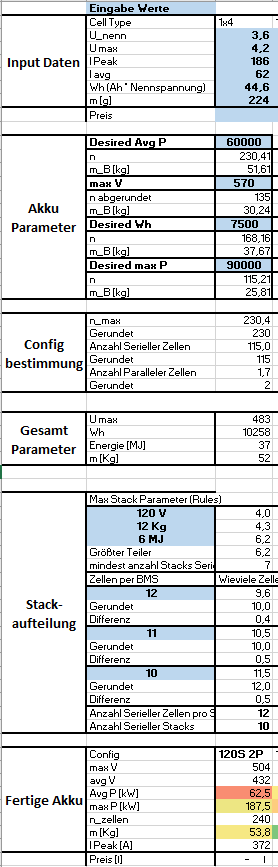
\includegraphics[width=0.2\linewidth]{bilder/Ausschnitt_zellvergleich}
	\caption{}
	\label{fig:Ausschnitt_zellvergleich}
\end{figure}
\FloatBarrier
Unter dem Punkt Input Daten werden die Zellparameter aus dem Datenblatt der Zelle angegeben. Unter den Akkuparametern werden nun die Zielbgedingungen bzw, Grenzwerte für den Akku Bestimmt. Die min Avg. P. ist hierbei ein Parameter für die im endurance angestrebte leistung, die max.V ergibt sich aus der sapnnungsfestigkeit des TS besonders relevant sind hierbei die Elektromotoren. Die min Wh geben die mindest vorgesehene akkukapazität vor und die min max. P. die angestrebte maximale leistung die der akku können muss. Aus diesen parametern wird folgend eine minimal benötigte Zellanzahl bestimmt. Unter dem Punkt Akkuconfig wird nun die vorhgerig höchstze bestimmte zellanzahl ermittlewt und gerundet. hieraus bestimmen wir nun die Anzahl der parallel und seriell verschalteten zellen und runden auf ganze zellen.
Dies ergibt dann einige Gesamtparameter für den akku.
Unter dem Abschnitt stackaufteilung werden die zellen jetzt nach den parametern des Regelwerkes möglichst optimal in stacks aufgeteilt. Der zielwert hierbei ist es das die tatsächliche Anzahl an Akkuzellen größer ist als die vorher errechnete benötigte Anzahl, es wird also aufgerundet. Weiter soll möglichst eine gerade anzahl an stacks heauskommen so das sich die stacks im akku möglichst leicht verteilen lassen. Hierbei können wir drei verschiedene anzahlen von zellen pro BMS vorgeben die analysiert werden sollen.
Schlussendlich ist das ergebnis ein fertig konfiguirierter akku. Diese konfigurationen können nun gegenübergestellt und die anzahl der weiter zu analysierenden zellen eigegrenzt werden.

Zur weiteren Analyse wurde auf Messdaten zurückgegriffen welche auf den Seiten dampfakkus.de und lygte-info.dk bereitgestellt wird. Aus diesen Daten ergeben sich folgende 2 Diagramme.
\begin{figure}[h]
	\centering
	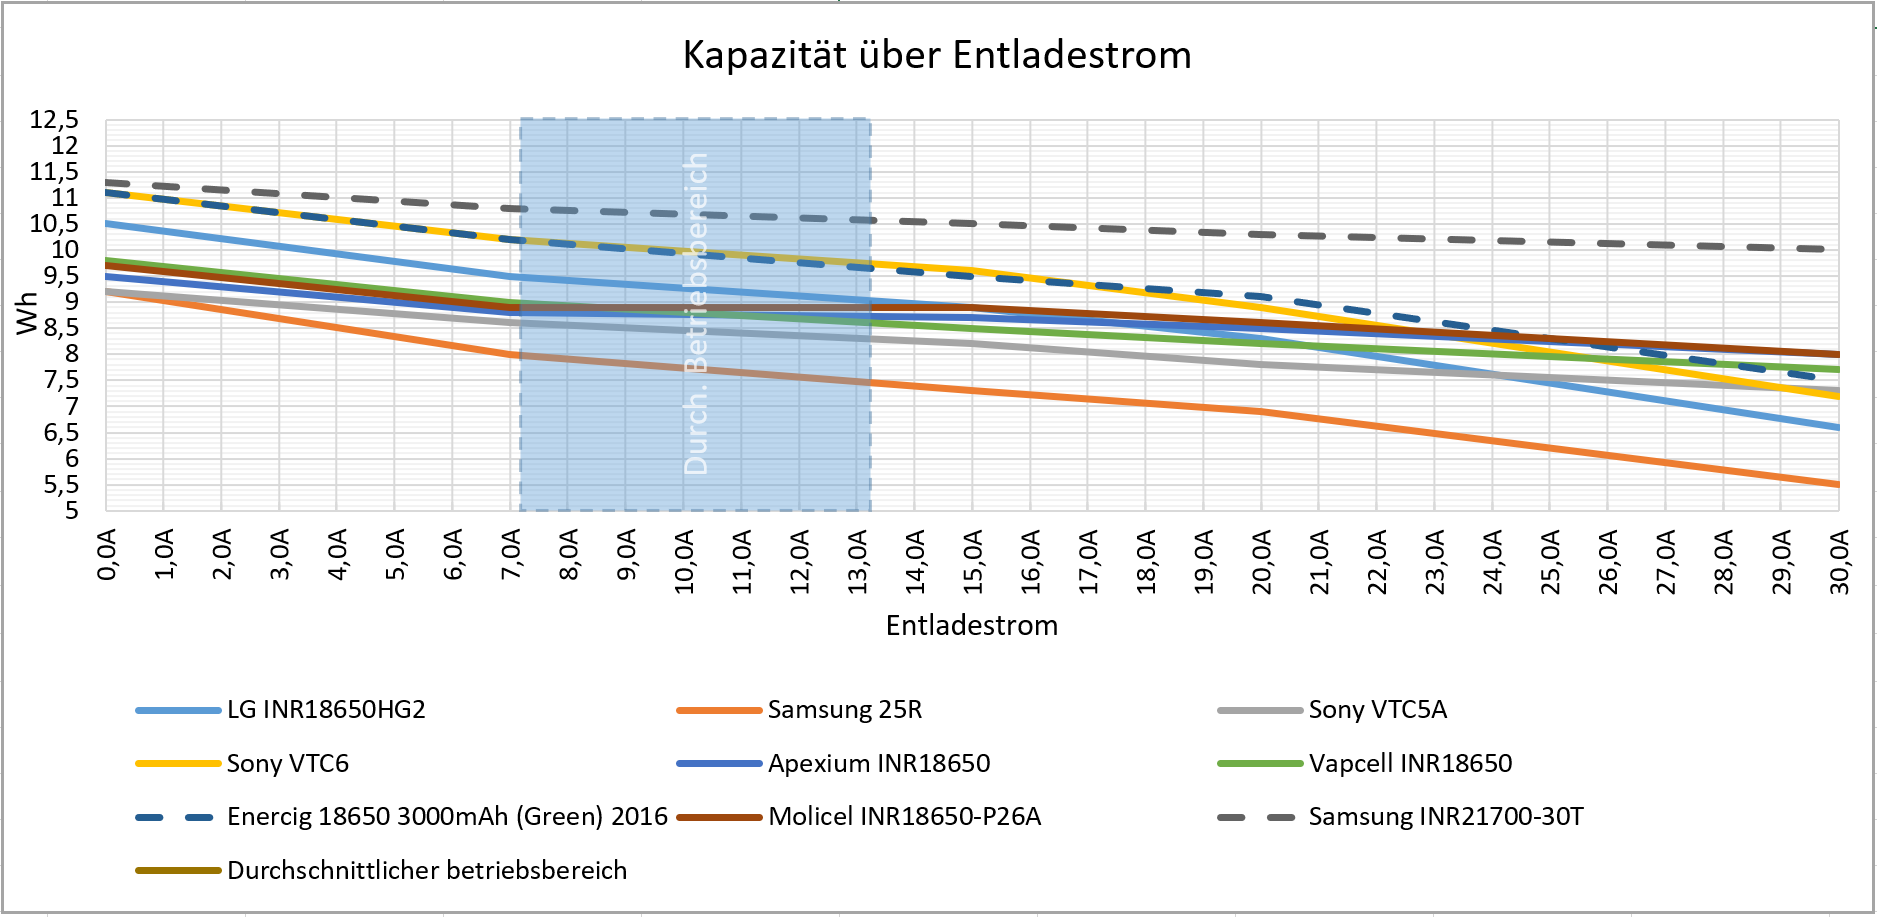
\includegraphics[width=0.6\linewidth]{bilder/Kapazitaet_ueber_Entladestrom}
	\caption{}
	\label{fig:Kapazitaet_ueber_Entladestrom}
\end{figure}
\begin{figure}[h]
	\centering
	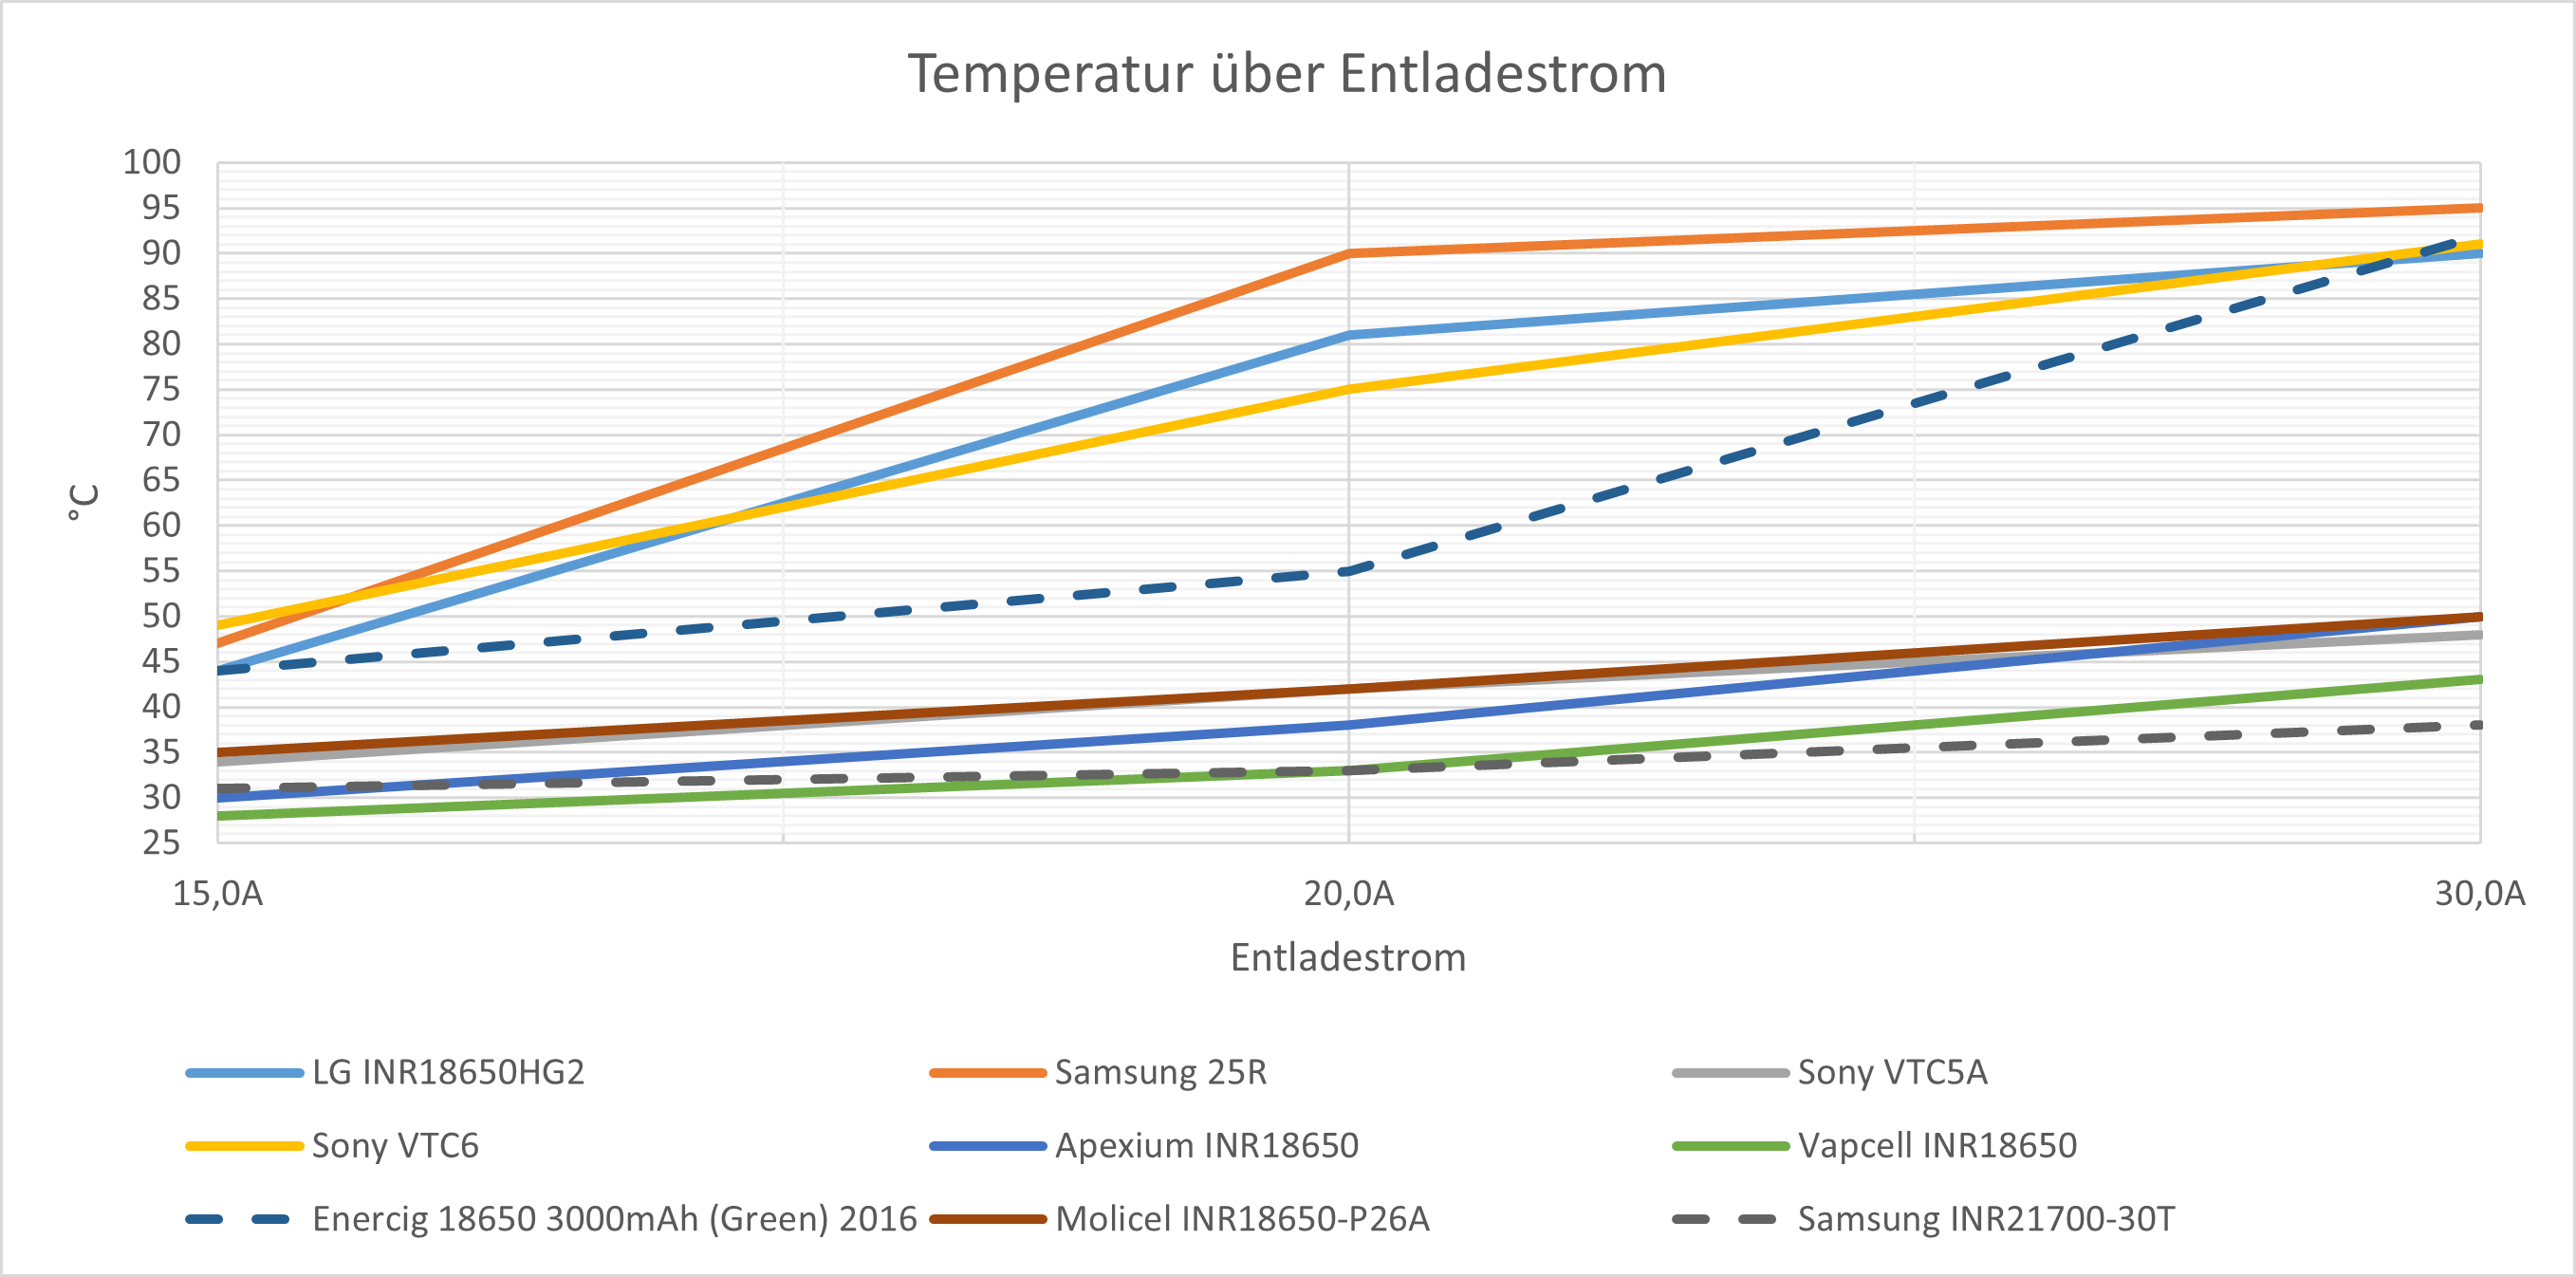
\includegraphics[width=0.6\linewidth]{bilder/Temperatur_ueber_Entladestrom}
	\caption{}
	\label{fig:Temperatur_ueber_Entladestrom}
\end{figure}
Das erste Diagramm ermöglichts es einen eindruck von der Entlladeeffizienz des Akkus besonders bei hohen Strömen zu bekommen. Das Optimum wäre hier eine Horizontale Linie am oberen Rand des diagrammes. Hierbei sticht die Samsung INR21700-30T besonders hervor.
Das zweitere Diagramm ermöglich uns einen eindruck von der thermischen performance zu erlangen. Laut regelwerk der Formula Student darf keine akuzellen zu einem Zeitpunkt die 60°C marke überschreitern. Nichtbeacjten führt zur disqualifikation. hierbei sticht auch die vorher genannte samsung zelle hervor als auch die Vapcell INR18650
Hierbei vergleichen wir Rundezellen von verschiedenen Baumaßen, ein Vollständiger akku mit den Samsung INR21700-30T wäre 7Kg schwerer als einer mit der Sony VTC6. Daher müssen am ende alle erlangenden Erkenntnisse Berücksichtigt werden.

%evtl. netzgrafik von den top 2 oder 3 zellen machen. als finale gegenüberstellung 
\FloatBarrier
\subsubsection{Elektrisches Modell der Zelle}
Das Elektrische Modell ist für die modellierung in der Rundenzeitsimulation relevant. Hierbei werden die limitierungen die sich aus dem Akku und dem restlichen antriebsstrang ergeben mit simuliert ein beispiel ist die sinkende antriebsleistung bei abfallen der spannung durch sinkenden SOC. Das aktuelle modell greift dabei auf zwei datensätze zu um das verhalten zu modellieren. Einmal die Entladeeffizienz bzw. einen korrigierten entladestrom, als auch auf ein Spannungskennfeld über entladestrom und SOC. Beide Abbildung folgen für die Sony VTC6. Die Daten entstammen wieder der Webseiten dampfakkus.de und lygte-info.dk.
\begin{figure}[h]
	\centering
	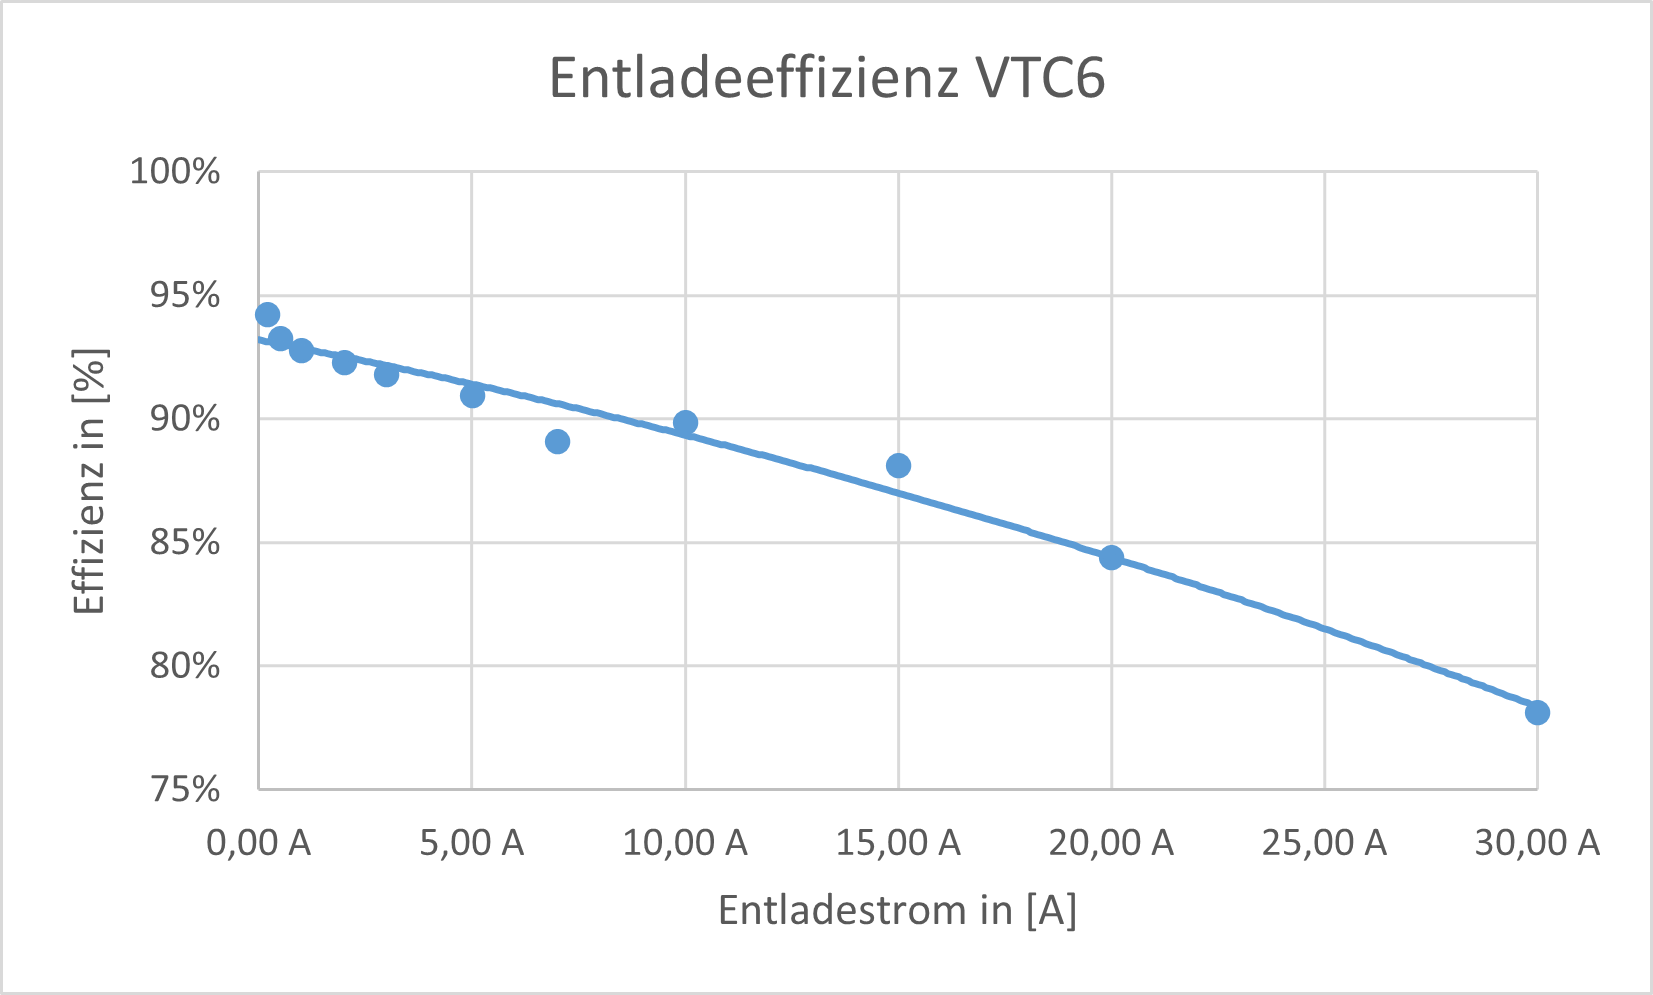
\includegraphics[width=0.7\linewidth]{bilder/Entladeeffizienz_VTC6}
	\caption{}
	\label{fig:Entladeeffizienz_VTC6}
\end{figure}
\begin{figure}[h]
	\centering
	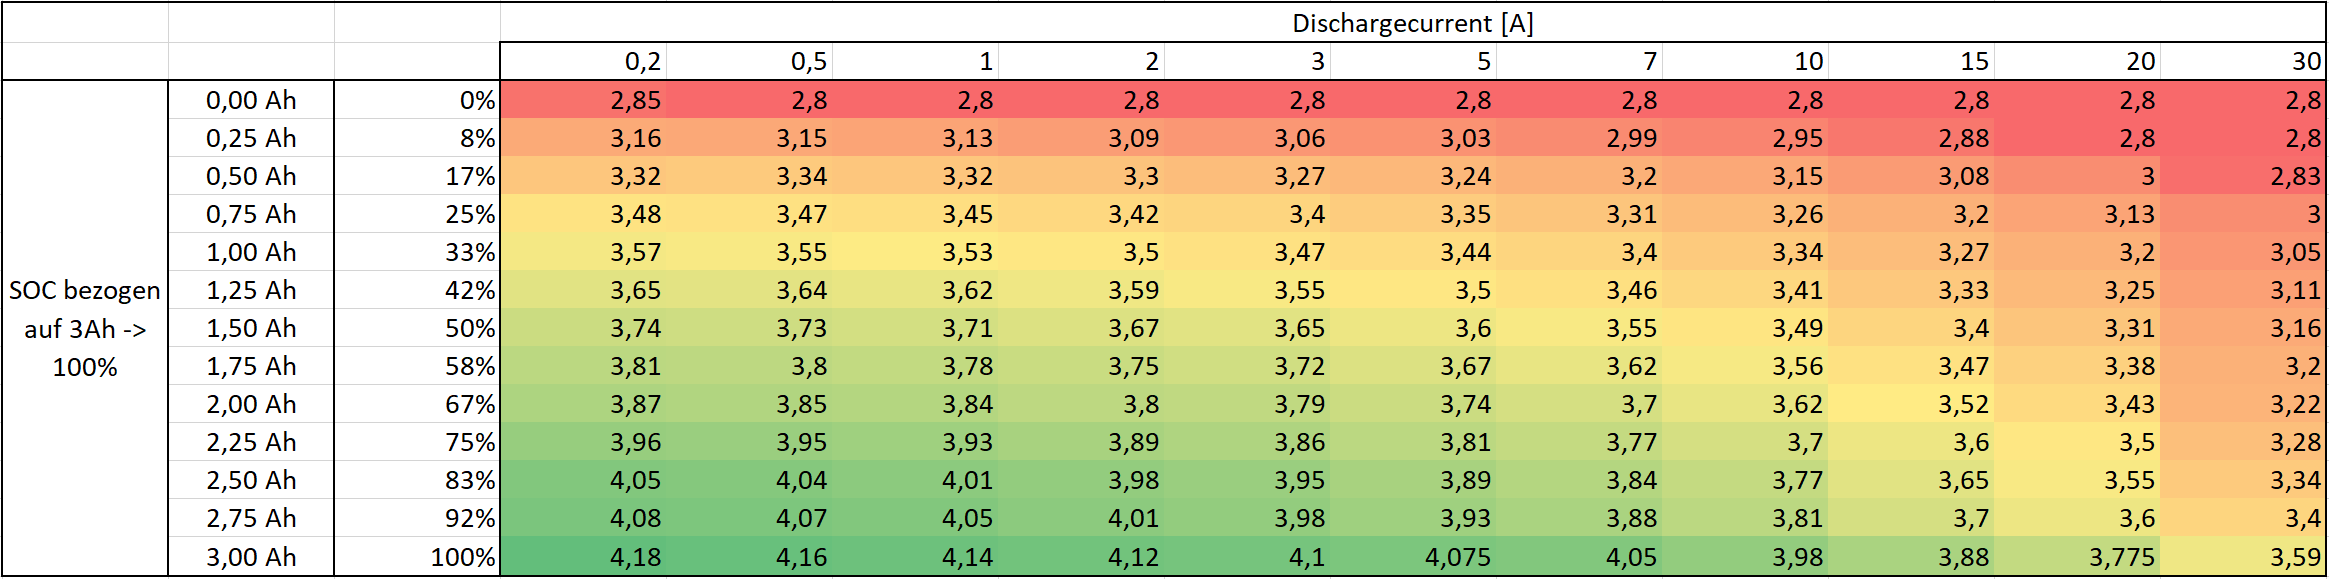
\includegraphics[width=0.7\linewidth]{bilder/Spannung_ueber_SOC_Strom}
	\caption{}
	\label{fig:Spannung_ueber_SOC_Strom}
\end{figure}

\subsubsection{Temperaturmodell der Zelle}

Auf Basis der Masterarbeit Experimentelle Untersuchung von Batteriesystemen im simulierten niedrigen Erdorbit von Agnes Klein an der Universität Stuttgart konnte ich ein simples thermisches modell der akkuzelle in einer excel tabelle ersytellen. Bei dieser arbeit wurde unter anderem die akkuzellen des types VTC6 innerhalb einer thermnal vakuum kammer betrieben und die thermischen paramter der zelle ermittelt. In folgender Grafik finden sie die dabei ermittelten parameter.

\begin{figure}[h]
	\centering
	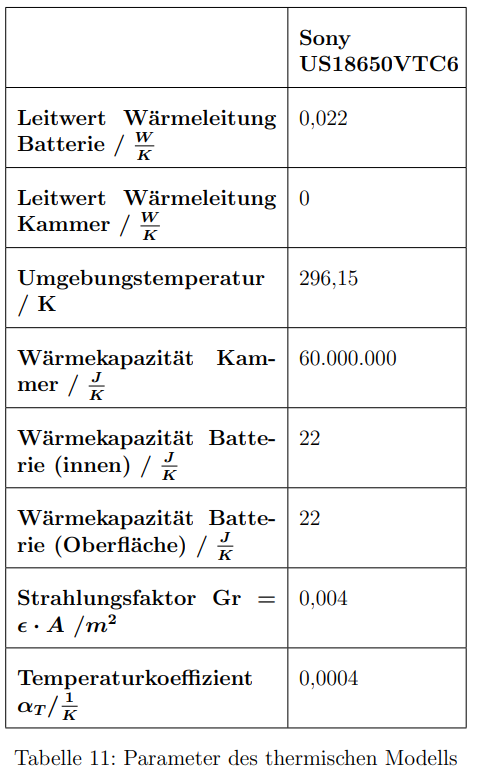
\includegraphics[width=0.4\linewidth]{bilder/Parameter_thermisches_modell_VTC6}
	\caption{}
	\label{fig:parameterthermischesmodellvtc6}
\end{figure}


Damit ergibt sich folgendes Modell.

\begin{equation}
	\glsc{symb:T_celli+1} = (\glsc{symb:I_cell}^2 * \glsc{symb:R_cell} - \glsc{symb:G_th} * (\glsc{symb:T_celli} - \glsc{symb:T_u}) - \glsc{symb:G_r} * \glsc{symb:SBoltz} * (\glsc{symb:T_celli} - \glsc{symb:T_u})^4) * \dfrac{1}{\glsc{symb:C_B} * \glsc{symb:m_Cell}} + \glsc{symb:T_celli}
\end{equation}

Mit diesem Modell ergeben sich folgende Kurvenverläufe für eine Auswahl Entladeströmen

\begin{figure}[h]
	\centering
	\includegraphics[width=0.7\linewidth]{bilder/temperatur_über_energie_vtc6_thermo_modell}
	\caption{}
	\label{fig:temperaturuberenergievtc6thermomodell}
\end{figure}

Mithilfe der folgenden Grafik von der Universität BRNO (MATEC Web of Conferences 313, 00045 (2020)) können wir einen Plausibilitätscheck durchführen. Wir haben hier Messdaten von der Sony VTC6. hierbei sind jedoch die Testbedingungen unbekannt. Als grobe Abschätzung sollte dies jedoch ausreichen

\begin{figure}[h]
	\centering
	\includegraphics[width=0.7\linewidth]{"bilder/Messdaten_VTC6_ temperatur kapazität spannung"}
	\caption{}
	\label{fig:messdatenvtc6-temperatur-kapazitat-spannung}
\end{figure}

Wir sehen das das erstellte modell für den 10A graph um ca. 3°C abweicht. Weiterhin sehen wir das bei der 20A linie die 90°C ca. 0,5Ah früher erreichen. Diese Abweichungen nicht insignifikant, zeigen jedoch das unser modell eher zu hohe als zu niedrige temperaturen ausgiebt was für die zuverlässigkeit des fahrzeuges positiv ist da eine auslegung der kühlung mit diesem modell wahrscheinlich zu einer überkühlung und damit zu einem zu hohen gewicht des kühlsystemes führt was für das erste fahrzeug kein sonderliches problemn darstellt. Die abweichung dürfte darauf zurückzuführen sein das die modellparameter im vakkum ermittelt worden und insofern wärmeübertragung durch konvektion etc. nicht berücksichttigt werden konnte. Um diesem sachverhgalt weiter auf die gründe zu gehen wurde im anschluss eine Simulation mit ansys fluent durchgeführt.

\begin{figure}[h]
	\centering
	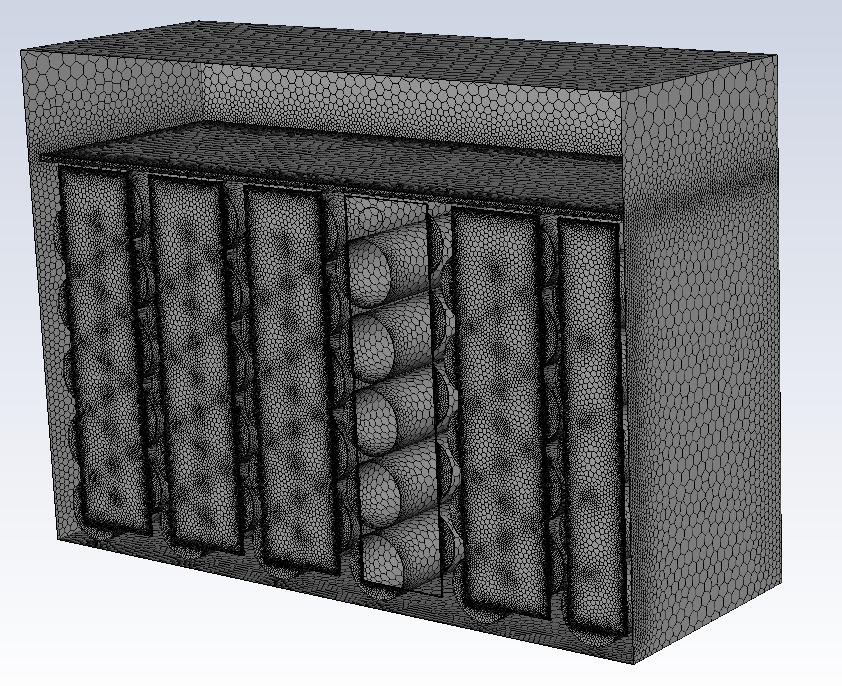
\includegraphics[width=0.7\linewidth]{bilder/Accu_Sim_therm_7_2A_45min_simple_mesh}
	\caption{}
	\label{fig:accusimtherm72a45minsimplemesh}
\end{figure}

\begin{figure}[h]
	\centering
	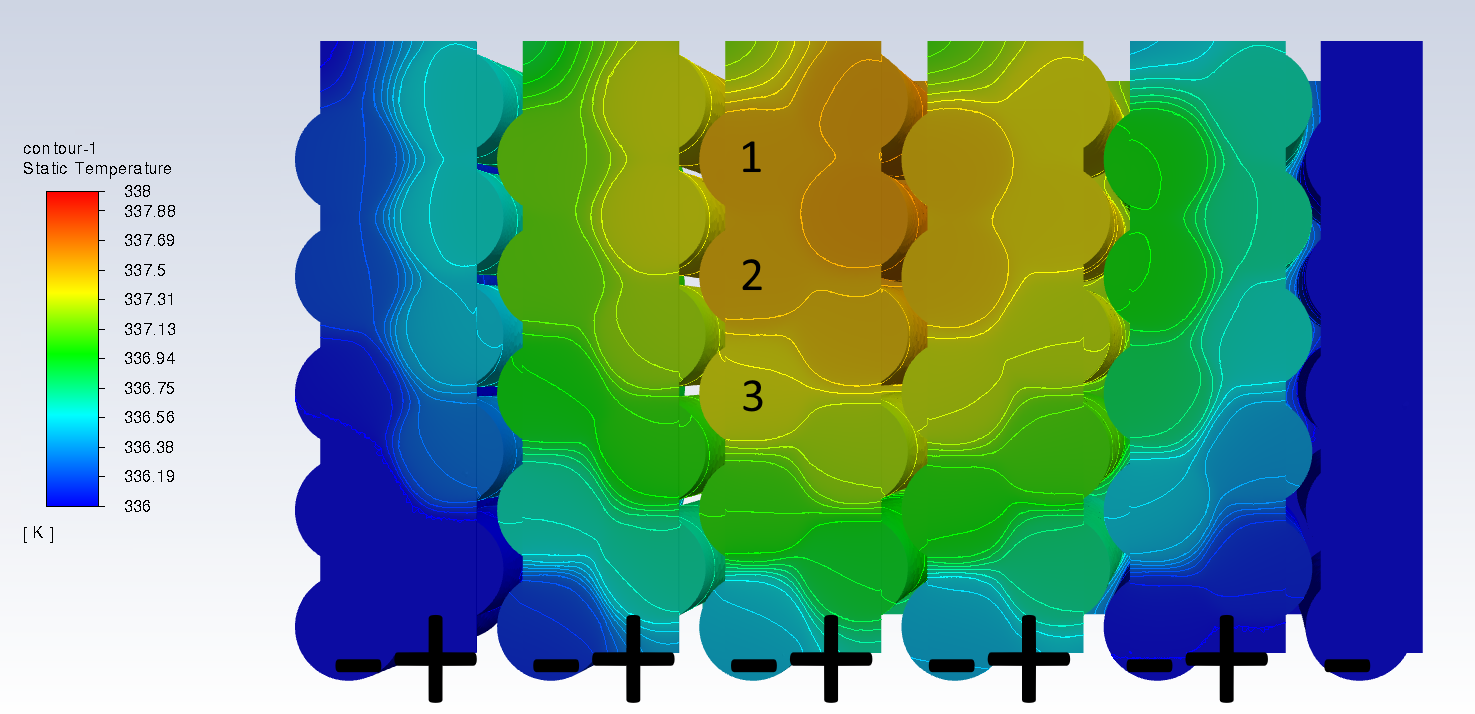
\includegraphics[width=0.7\linewidth]{bilder/Accu_Sim_therm_7_2A_45min_simple}
	\caption{}
	\label{fig:accusimtherm72a45minsimple}
\end{figure}

In dieser simulationb wurde ein gesamter akkustack in seinem gehäuse simuliert. dabei wurde mit einem konstanten strom von 7,2A simuliert. Dieser strom ergibt sich aus der rundenzeitsimulation siehe sectrion. Die Simulation wurde für 32min laufen gelassen um eine gesamtes endurance darzustellen. Ziel der simuzlation ist es die effekte der konvektion zu berücksichtigen aber auch zu sehen in wiefern sich die zellen gegenseitig beeinflussen. Allerdings wurden auch diverse vereinfachungen getroffen insofern das die akkuzellen sich uniform aufwäremn. In der realität dürfte man am negativen pol der akuzelle eine deutlich höhere temperatur feststellen könne als auf der positiven seite. weiterhin wurden diverse teile wie die elektrische isolierung etc. weggelassen da dies den simulations aufwand sonst erheblich vergrößert hätte und die simulation so schon 2 tage benötigt hat. zur analyse, wir sehen nach der simulationszeiot eine hot spot temperature von 64,85°C und eine niedrigste temperatur von 62,85°C. In dieser hinsicht stimmt die ansys simulation eher mit der 10A kurve aus unserem modell zusammen als mit den messdaten. Zusammengefasst stellt man fest das definitiv weitere arbeit in diesem themenbereich von nöten wäre um zu einer optimalen lösung zu kommen dies jedoch aufgrund des engen zeitplanes und des enoremn anderweitigen aufwandes nicht möglich ist.
\FloatBarrier

\subsubsection{Der Stack Aufbau} %(mit Tim)%

Für die konstruktion des Akkustacks gab es im Laufe der Saison viele Iterationen. Die folgend erläuterte ist eine Optimierte Version derer die für den TY22 gebaut wurde.

\begin{figure}
	\centering
	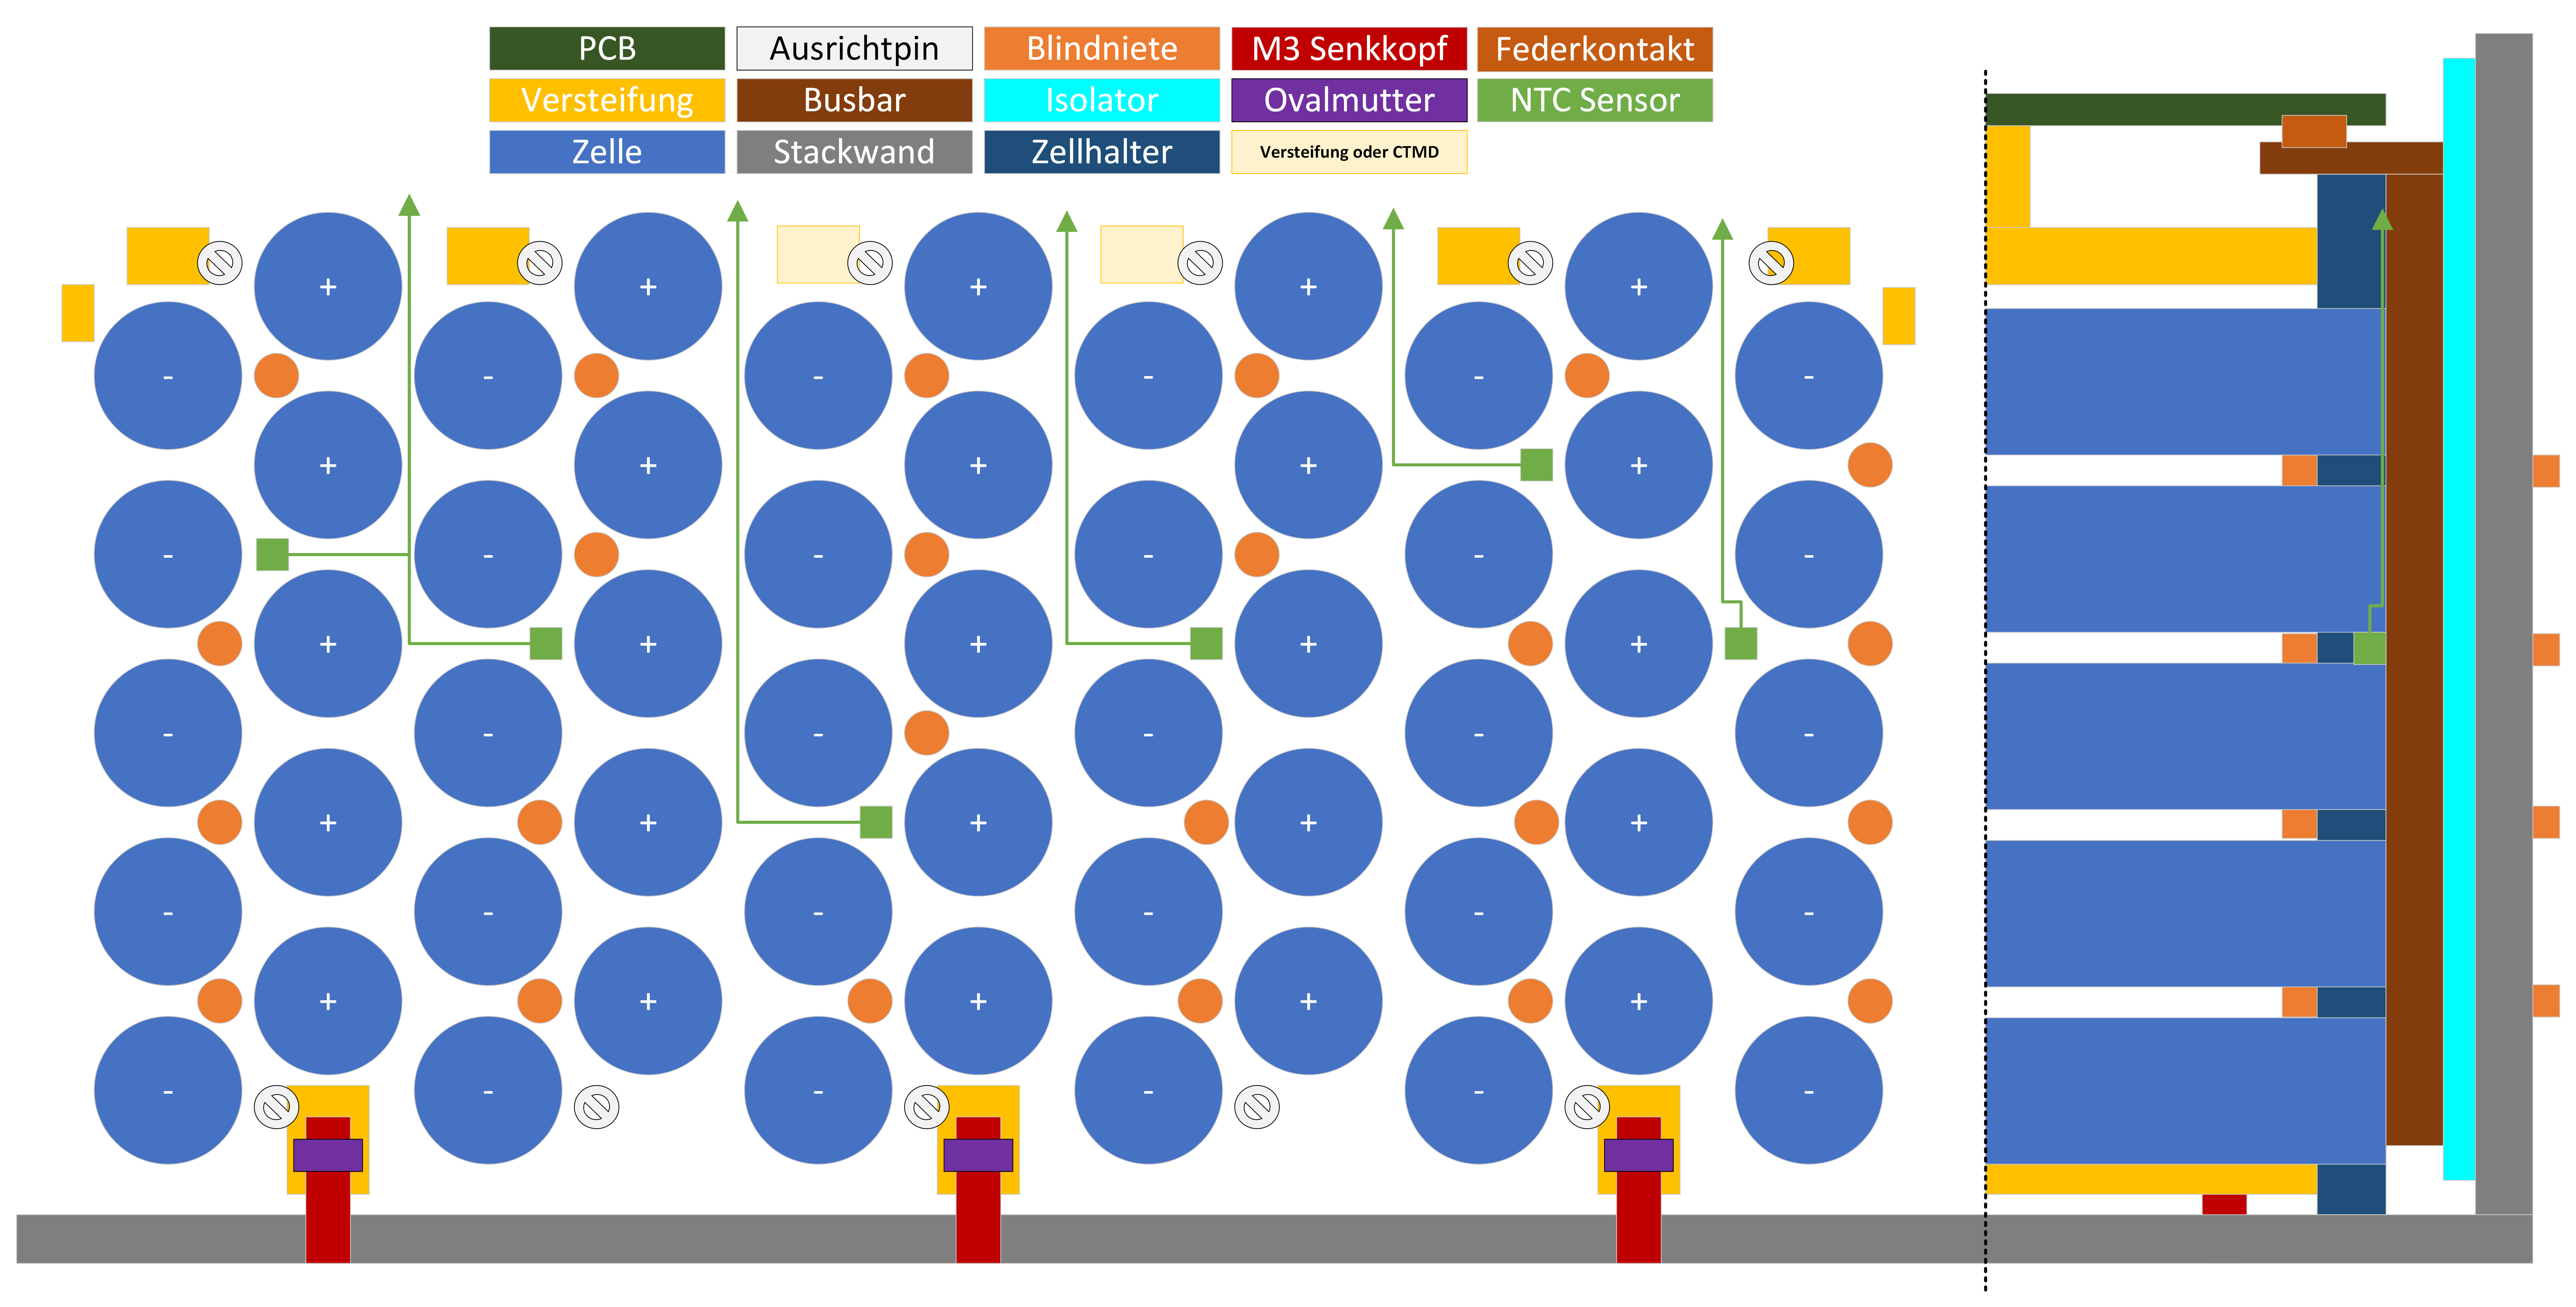
\includegraphics[width=0.7\linewidth]{bilder/Stackaufbau_Prinzipskizze}
	\caption{}
	\label{fig:stackaufbauprinzipskizze}
\end{figure}

Die zellen sind liegend in fünfer packeten gestapelten und mit einem versatz aneinander gereiht um den leerraum zwischen den zellen möglichst lein zu halten. Die Busbars verbinden immer ein 5er Negativpole mit einem 5er positiv pole. Zusätzlich befinden sich in der näöhe der zellen 2 ausrichtpins um die busbar auf dem stack bei der montage positionieren zu können. Der aufbau auf dn Polen besteht aus einer angeschweißten Busbar, darauf folgt ein abriebfester isolator, und dann eine trennwand des akkus. nach innen haben wir noch einen 3D gedruckten Halter in dem die Akuzellen ausgerichtet werden. Dieses ganze paket wird mit blindnieten vernietet. Ziel hierbei ist es einen möglichst guten thermischen kontakt von den Polen der Zelle zum Akkugehäuse herzustellen. Selbiges ist aus aluminium und Flächig mit dem Monocoque verschraubt welches auch aus aluminium gefertigt ist. dies ergibt eine riesige thermische masse und stellt so eine Kühlung für den akku bereit. Die stack seitenwand liegt als L-Profil vor, und wird anschließend mit demm akkuboden mit hilfe von M3 Senkkopfschrauben und Ovalmuttern verschraubt. In diesem zuge sind in die 3D gedruckten querversteifungen im stack ovalmuttern eingeklebt. Diese querversteifung sorgen einerseits für mechanische stabilität, stellen aber auch anbindungspunkte für den AMS Slave als auch für die Maintenace Plug steckverbinder bereit. Die Busbar ist auch als L Profil ausgeführt und lappt oben über den Stack über, diese finnen werden seitens des AMS slaves mit hilfe von federkontakten kontaktiert um eine verbindung für die spannungsmessung als auch das balancing herzustellen. Die NTC sensoren befinden sich in den Leerstelln wo keine Nieten benötigt werden, immer eine Niete mittig in drei zellen. Sie sind rückseitig auf die Busbar geklebt. Um das design günstig zu halten kann die verbidnung kann über 0,35mm\^2 kabel erfolgen welche Sensor seitig auf Lötpads und AMS seitig in einen stecker gebracht werden. Bei der Steckverbinderauswahl hier ist zu achten das der er über einen verrigelungsmnechanismus verfügt, und nicht zu klein ist. Besonders kleine Steckverbinder machen an der stelle die verarbeitung schwer oder praktisch unmöglich. Präferiert wäre hier ein Flex PCB, dies ist jedoch idR. recht teuer. In dem Stackhalter müssen entsprechende Einkerbungen vorgehalten werden durch die die Kabel zu führen sind. In die anbindung des AMS Slave ist ein feature vizusehen welches eine leichte extraktion des stacks aus dem akku erlaubt, und bei der konstruktion der maintenance plugs ist auf ergonomie zu achten, so das ein mensch mit einem HV handschuh noch gefahrlos einen solchen ziehen kann. Weiter ist bei den maintenace Plugs auf verstecksicherheit zu achten. Ein letzter Punkt ist die positionierung des CTMD, also entweder des i button oder dieser kleinen kabelgebunden sensoren mit dem steuergerät, je nachdem was die FSG verwenden möge. Hier ist besonders die positionierung des CTMD am Hotspot schwer nachzuweisen. eine simualtion kann hier eine richtung aufzeigen, stellt jedoch einen großen zeitaufwand dar und ist im allgemeinen so ungenau (ohne signifikanten Zeitaufwand), dass sich nur sehr begrenzt belastbare aussagen hiermit treffen lassen.

\FloatBarrier

\subsubsection{Die Busbar}
Busbar material und dicken auswahl
 Bei der Auswahl der Materialien für die Busbar sind die Masse als auch die elektrische respektive die thermische Performance ausschlaggebend. Ein weiterer Maßgebender Faktor sind die möglichen Fertigungsverfahren um den Kontakt zwischen Zelle und Busbar herzustellen. Folgende Grafiken ergeben sich aus den Materialkonstanten und der Erwärmung über den widerstand der Busbar bei dem entsprechenden Strom und über die Wärmekapazität und die Betriebszeit.
 
 \begin{figure}[]
 	\centering
 	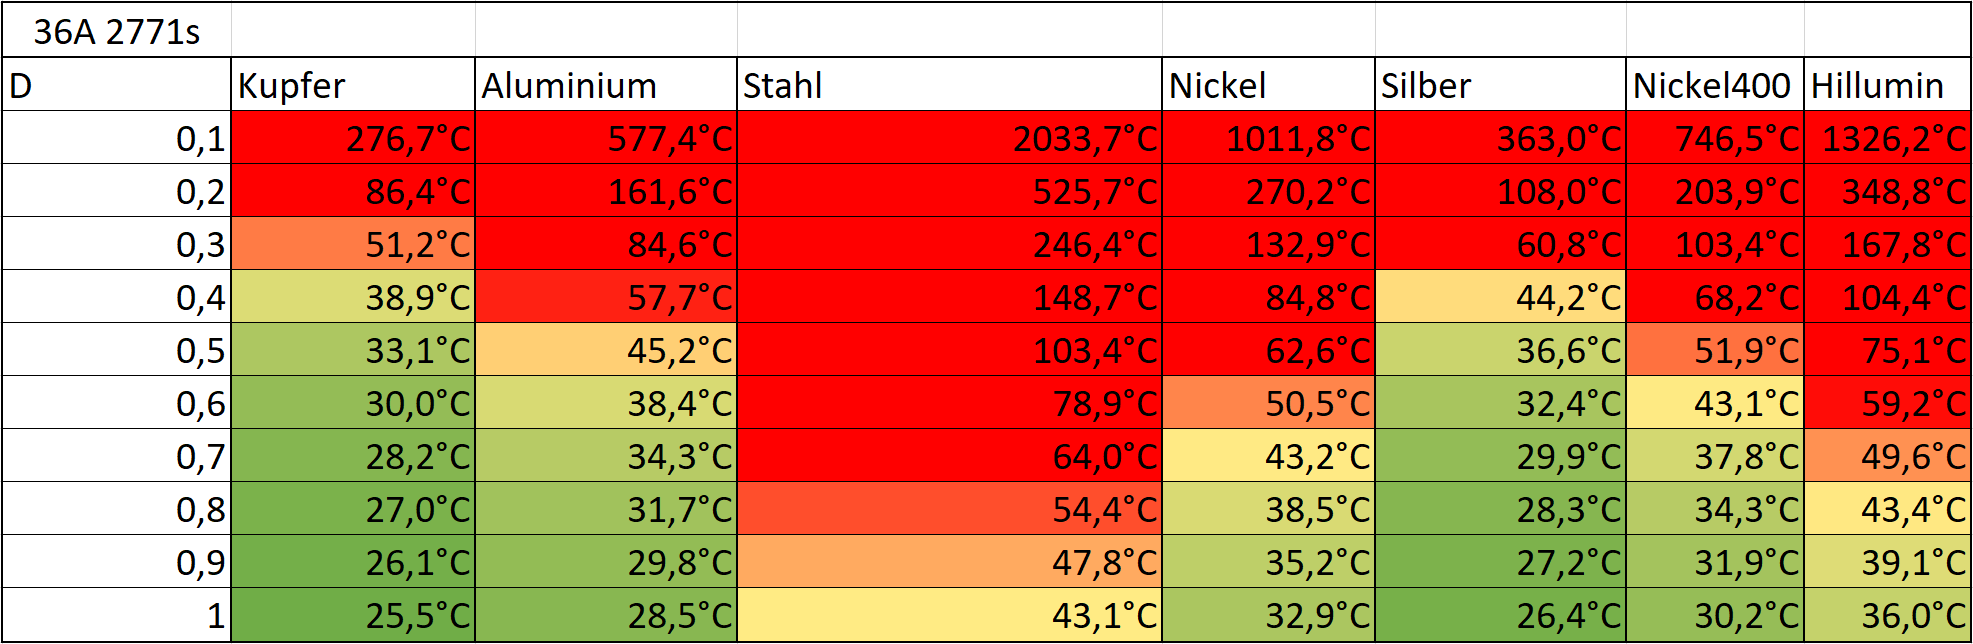
\includegraphics[width=0.7\linewidth]{bilder/Busbar_temp_36A_2771s}
 	\caption{}
 	\label{fig:Busbar_temp_36A_2771s}
 \end{figure}
\begin{figure}[]
	\centering
	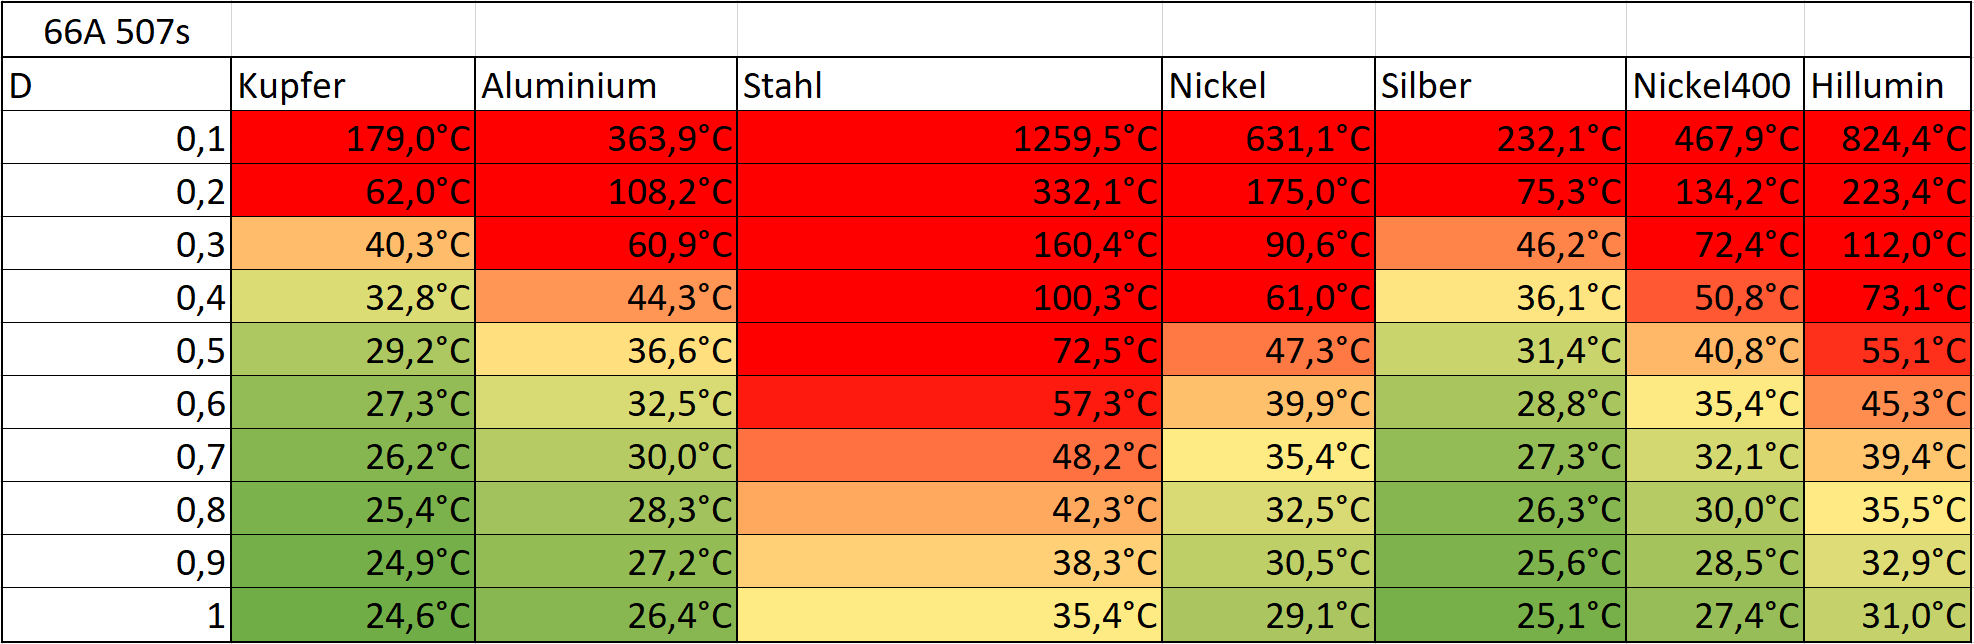
\includegraphics[width=0.7\linewidth]{bilder/Busbar_temp_66A_507s}
	\caption{}
	\label{fig:Busbar_temp_66A_507s}
\end{figure}
\begin{figure}[]
	\centering
	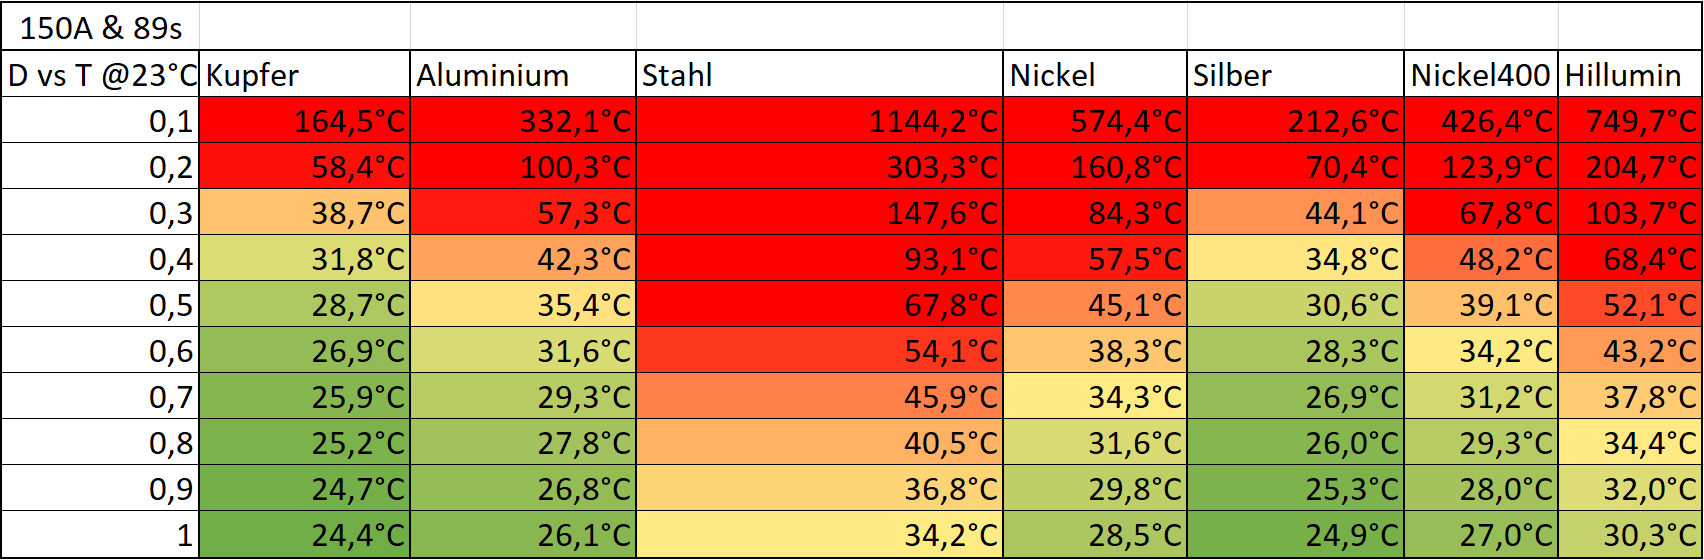
\includegraphics[width=0.7\linewidth]{bilder/Busbar_temp_150A_89s}
	\caption{}
	\label{fig:Busbar_temp_150A_89s}
\end{figure}

Es ist ersichtlich das Kupfer die beste thermische performance in bezug auf die materialmenge bringt, aufgrund der niedrigen dichte aluminium allerdings gravimetrisch mit abstand die beste perfromance zeigt. Nickel, respektive Nickel400 liegen jedoch nicht weit zurück, ledeglich stahl lässt sich aufgrund der ergebnisse direkt ausschließen.

In bezug auf die fertigung ergeben sich bei rundezellen zwei wege, einmal das schweißen aber auch die federkontaktierung.
Die Kontaktierung über eine feder an eine Rundzelle sollte dem Leser hinreichend aus anderen batteriebetriebenen Geräten hinreichend bekannt sein. Hierbei ergeben sich schnell einige Fragestellungen. Einmal die frage nach der Ermittlung des Übergangswiederstandes. Einflussfaktoren sind die Anpresskraft, die Oberflächenrauhigkeit, die Kontaktfläche, als auch der Materialmix. Eine Berechnung ist jedoch praktisch aufgrund des enormen Aufwandes und großer unsicherheitewn kaum möglich. Weiter stellt sich da die frage wie groß z.b die max. mögliche Anpresskraft auf die Akkuzelle sein kann oder welche oberflächenrauhigkeit eine Pol mit sich bringt. Weiter ist die Relaxation ein Problem. hierbei würde die Anpresskraft im verlauf der zeit abnehmen und damit der Übergangswiederstand steigen. All diese Parameter müssten in aufwendigen und langwierigen Versuchsreihen ermittelt und untersucht werden um auf ein sicheres System zu kommen. Das Verschweißen von Akkuzellen wird dabei gerade im Hochstrombereich bereits industriell angewandt und ist damit hinreichend bekannt. 
Bei den Schweißverfahren teilt sich nun der weg in das Laser bzw WIG schweißen und in das Punkt oder Wiederstandschweißen auf. Ersteres verfahren ermöglicht das verschweißen unterschiedlicher Metalle wie z.b Stahl an Aluminium oder Kupfer. Zweiteres Verfahren eignet sich nur für Materialien mit einem verhältnismäßig hohen elektrischen widerstand da der Schweißpunkt durch die Temperaturentwicklung gebildet wird die entsteht wenn ein hoher Strom durch einen verhältnismäßig hohen Übergangswiederstand geleitet wird. Daher eignet sich das Wiederstandschweißen nur für Nickel oder stahl. Die anderen Materialen sind nicht inhärent nicht geeignet, stellen aber besondere Anforderungen an den Prozess so das die Standard Geräte hier idr. nicht ausreichen. Systemparameter sind beim Wiederstandsschweißen die Schweißspannung als auch der Schweißstrom und die Pulsdauer. Ein großer Nachteil des Laser bzw. WIG Schweißens ist das dieses Verfahren bisher nur im industriellen Maßstab angewandt wird und es keinerlei Geräte für den Hobbybedarf gibt. Dies führt dazu das diese Geräte idr. enorm teuer und schwer zu bekommen sind. Hierbei wäre es sicherlich möglich ein typisches WIG Schweißgerät für diese Zwecke zu modifizieren dies bringt jedoch wieder die entsprechende Unsicherheit in den Prozess. Punktschweißgeräte sind in diversen Ausführungen und Preisklassen gut erhältlich und ermöglichen so einen Kostengünstigen einstieg.
	
\FloatBarrier
\subsubsection{Der Akkumulator Container}

Der akku besteht aus 12 einzelstacks. Hiewrbei befinden saich 6 nebenbeiander und davon 2 reihen hintereinander. in der vorderen sektion die unter den fahrersitz ragt befinmden sich die HV Relais als auch die übrige Akkumulator elektronik wier das IMD der AMS MAster und der HVDCDC.
\begin{figure}
	\centering
	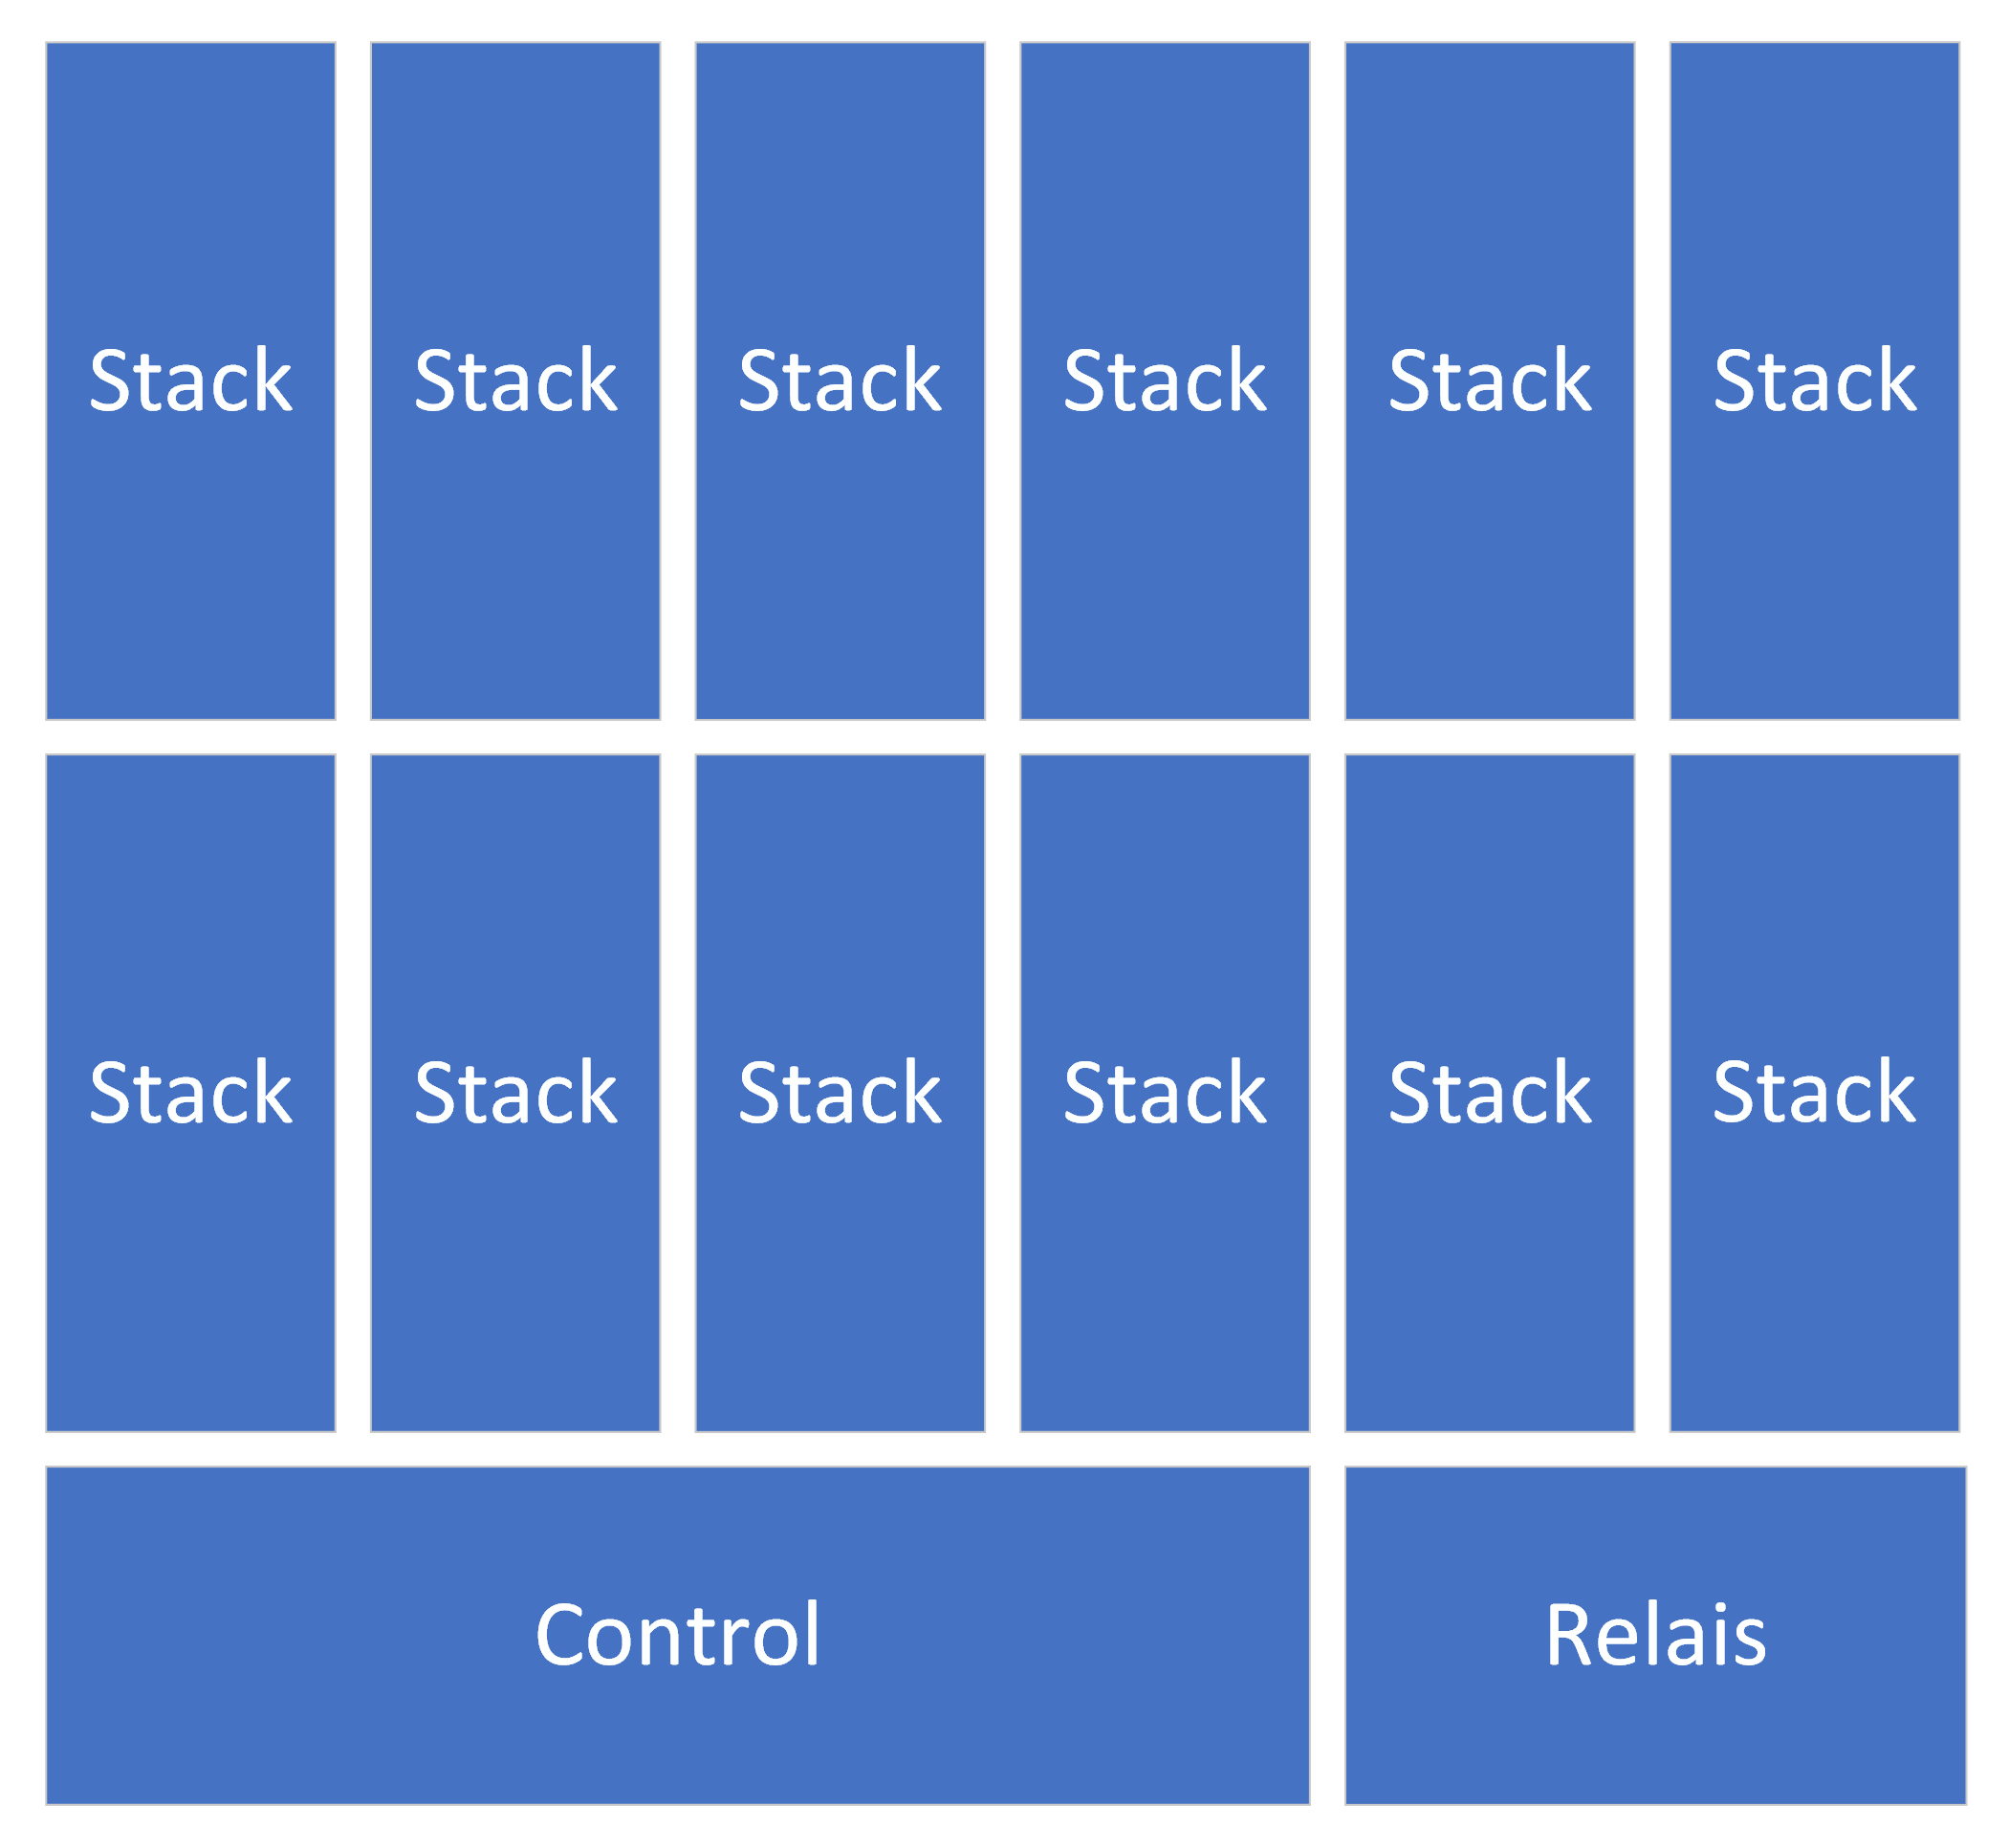
\includegraphics[width=0.7\linewidth]{bilder/Akku_Layout}
	\caption{}
	\label{fig:akkulayout}
\end{figure}
Der akkumulatorcontainer besteht aus aluminium. dabei muss vom regelwerk her der boden midnestens 3,2mm und die wände 2.3mm dick sein. gewählt wurden respektive 4mm und 2,5mm. In der ersten version handelt es sich bei dem container um mehrere geschweiste biegeteile, solches konstrukt zeichnete sich jedoch durch derart starken schweißverzug aus das bei der folgeversion eine kombination aus Nieten kleben, schrauben und schweißen anzuraten ist. gerade mit dem überarbeiten stack konzept lässt sich eine reine schweißkonstruktion nicht mehr umsetzten. Hierbei währen die Stackwände vernietet und verschraubt, die Bodenwanne eine biege-schweißteil, der deckel einbiegeteil und etwaige interne anbindung für z.b die HV stecker sind geklebt.

!!Bild von aktueller CAD mit beschriftung!!

\section{Elektromotor}
Im großen und ganzen gibt es für die Auswahl des Elektromotors 4 verschiedene in der Formula Student allgemein anerkannte Lösungen. Diese werden nachfolgend erläutert.

\subsection{Emrax}
Beim Emrax Motor handelt es sich um eine Axial Flux Permanent erregte synchron Maschine PMSM. zusammenfassend sind die emrax motoren sehr flacj haben aber einen großen durchmesser. Sie zeichnen sich durch ein hohes drehmoment und damit verhältnismäßig niedrige drehzahlen aus, im bereich von 7-8K RPM. Sie sind nur in recht großen formaten und damit großen leistungen erhältlich so das ein 1 oder 2 motoren antriebskonzept realisierbar ist. Außerdem handelt es sich hierbei um eine reine kauflösung. 

\subsection{AMK}
Die AMK motoren sind radial flux PMSM. Sie sind insofern eher lang und haben kleine druchmesser. Die bauform gleicht insofern eher dem klassischen elektromotor. Sie zeichnen sich durch extrem hohge drehzahlen aus, oberhalb der 20k und damit durch eine enorme leistungsdichte. Sie sind in eher kleinen leistungsdichten zu bekommen so das beinahe nur ein Allrad antrieb sinnvoll umsetzbar ist. Auch hierbei handelt es sich um eine reine kauflösung. 

\subsection{Fischer}
Die Motoren von fischer sind im großen und ganzen gleichzusetzten mit den amk motoren. der große unterschied ist das hier das gehäuse selbst designt werden muss und alle teile selber gefertigt werden müssen. Die stellt große herausfordferungen die fertigungstechnik da es sich dabei auch um 5 achs gefräst6e titanteile handelt. 

\subsection{China \& Co}
Eine weitere Optionen wäre es gunstige motoren eines Chinesischen hersteller zu beschaffen, als bsp. wäre hier die firma Freerchhobby zu nennen, es gibt aber viele mehr. Diese motoren zeichnensich durch ein herausragend niedrigen preis hervor sowohl für den motor als auch den zugehörigen motorcontroller. Problematisch hierbei ist, das diese motoren iun der regel nur bis spannungsbereiche von 120V verfügabr sind. und der dabei bei 80kW resultierende strom enorm ist. Heißt das entweder die leistung zu reduzieren wäre oder die elektrische des auslegung des TS besondere anbsprüche gestellt hätte. Weiter stellt sich hier die frage der zuverlässigkeit. Vor nicht allzu langer zeit ist man im raciung team einen einzilindermtor dder firma borossi gefahren welcher sich durch nicht vorhandene haltbarkeit auszeichnete und so 3 saisons in folge torpedierte. Daher sind die anderen oiptionen sovern erwschwinglich vorzuziehen. sollte das Budget aber besonders eng sein, können diese motoren allerding durchaus eine valide alternative darstellen

\subsection{Selbstbau}
Der selsbtbau ist quais die nächste entwicklungsstufe nach dem fischer motor. Nun gilt es nicht nur den motor selber zu fertigung sondern auch die gesamte vorauslegung zu machen. es gibt nur wenige teams die einen selbstbau wagen, und noch werniger die es erfolgreich umsetzten.

\subsection{Entscheidungsfindung}
Die Entscheidung ist an diesem Punkt sehr einfach. Im rahmen dieser projektabreit entsteht der erste e antrioerb aus dem hause baltic racing. damit kommen enrom viele große heruasforderung. das heißt man sollte entweder die einfachste oder die nächst einfachste Lösung nehmen um am ende zu dem ziel des fahrenden autos zu kommen. Und da sich nur der emrax motor effektic für einen zwei rad antrieb eignet ist es der emrax motor gewotrden.

\section{Wechselrichter}
Der wechselrichter wird benötigt um den motor sauber anzusteuern. Ziel ist es aus gleichstrom aus dem akku einen Frequenz und amplituden regelbaren strom zu erzuegen mit dem der motor kontrolliert werden kann. Hier gibt es auch wieder diverse hersteller die im folgenden verglichen werden sollen

!!!Tabelle!!! mit daten

\section{Kabelbaum} (zusammen mit Nico Bieberich)
Die Entwicklung des Kabelbaumes erfolgt in der regel recht früh im entwicklungsprozess und zieht sich recht lange, da fast jede änderung an den elektrischen systemen auch eine änderung am kabelbaum nachsichzieht. Der kabelbaum lässt sich bei einem elektrofahrzeug iun mehrere funktionsgruppen unterteilen. Einmal haben wir den Datenbuss zur kommunikation der Steuergeräte im Fahrzeug. In unserem fall ist das ein CAN Bus. Dann den sogenannten Shudown circuit zur absicherung der systeme bzw. einleiten eines sicheren zusatendes in dem fall das ein fehler auftritt. Weiter gibt es die gruppe der Hochvolt kabel dies umfasst leistungsführende leiter für akku inerter und Motor als auch HV signalleiter für z.b. die TSMP. Dann haben wir noich die LVS Versorgung für alle systeme im Fahzeug. Dann gibt es den Sensor baum dieser umfasst die versorgungs als auch datenleitungten für jegliche sensorik im fahrzeug  Abschließend gibt es noch alles andere was sich nicht hierunter kategorisieren lässt. Dies umfasst z.b einzelne analoge oder digitale datenleitungeng wie z.b die Ethernet Leitung für den FSG Logger oder die Abzweigleitung des Bremsdruckes für das BSPD. Auf die einzelnen gruppen wird im folgenden detailiert eingegangen.\\
\\
Wichtige generelle Überlegungen beim Kabelbaum sind jegliche Maßnahmen die den Kabelstrang DAU sicher machen. Sprich verpolsichere steckverbinder Belegung der stecker so das ohne verpolschutz kein kapitalschaden eintritt. sauber logische farbcodierung sowohl der Kabel als wenn möglich auch der Steckverbinder sodass beim zusammenbau keine fehler gemacht werden und dies einheitliche am besten über jahre durchgängige durchgeführt.

Verpolschutz, richtige pins auf heiß0er seite, etc. etwas mehr ausführen

\begin{tabular}{|c|c|c|c|c|c|}
	\hline
	\multicolumn{6}{|c|}{Steckertypen} \\
	\hline
	Name & W2W/W2B & Montage & Sealed & Einsatzbereich & Pinanzahlen \\
	\hline
	Molex Micro Fit & both & Wire & no & HV/LV & 2-20 \\
	\hline
	Molex CMC/CMX & W2B & Panel & Yes & LV  & 28-154 \\
	\hline
	TE HD10/20/30 & both & both & Yes & HV & 3-47 \\
	\hline
	Molex Mizu P 25 & W2W & Wire & Yes & LV & 2-4 \\
	\hline
	Binder Sub M9 & both & both & Yes & LV & 2-8 \\
	\hline
	Binder M12 Power & both & both & Yes & HV & 2-8 \\
	\hline
	Würth WRBHD2.54 & W2B & Wire & No & LV & 10 \\
	\hline
\end{tabular}

\begin{minipage}{8cm}
\begin{tabularx}{8cm}{|c|c|}
	\hline
	\multicolumn{2}{|c|}{\textbf{\large {Farbtabelle}}} \\
	\hline
	Farbe & Signal \\
	\hline
	\multicolumn{2}{|c|}{\textbf {Kabel}} \\
	\hline
	White & 24V \\
	\hline
	\cellcolor{brown!30} Brown & GND \\
	\hline
	\multicolumn{1}{|@{}X@{}|}{\tikzmark[a]{Brown Green}} & CANH/Signal\\
	\hline
	\cellcolor{yellow!30} Yellow & CANL/5V \\
	\hline
		\hline
	\multicolumn{2}{|c|}{\textbf {Leiter}} \\
	\hline
	White & 24V \\
	\hline
	\multicolumn{1}{|@{}X@{}|}{\tikzmark[b]{White Yellow}} & 5V\\
	\hline
	\multicolumn{1}{|@{}X@{}|}{\tikzmark[c]{White Pink}} & 12V\\
	\hline
	\multicolumn{1}{|@{}X@{}|}{\tikzmark[d]{White Red}} & 3V\\
	\hline
	\cellcolor{brown!30} Brown & GND \\
	\hline	
	\cellcolor{green!30} Green & CANH \\
	\hline
	\cellcolor{yellow!30} Yellow & CANL \\
	\hline
	\cellcolor{blue!30} Blue & SDC \\
	\hline
	\multicolumn{1}{|@{}X@{}|}{\tikzmark[e]{Blue Red}} & SDC\textsubscript{end} \\
	\hline
	\multicolumn{1}{|@{}X@{}|}{\tikzmark[f]{Blue White}} & SDC\textsubscript{indicator} \\
	\hline
	\cellcolor{violet!30} Voilet & Signal \\
	\hline
		\hline
	\multicolumn{2}{|c|}{\textbf {HV-Leiter}} \\
	\hline
	\cellcolor{red!30} Red & TSMP+/HV+ \\
	\hline
	\cellcolor{black!30} Black & TSMP-/HV- \\
	\hline
	\cellcolor{blue!30} Blue & SDC \\
	\hline
		\hline
	\multicolumn{2}{|c|}{\textbf {Mehrader}} \\
	\hline
	\cellcolor{yellow!30} Yellow & LAN \\
	\hline
\end{tabularx}

\begin{tikzpicture}[remember picture,overlay]
	\path[fill=brown,opacity=0.3](a.north west)--(a.south west) -- (a.south east) -- cycle;
	\path[fill=green,opacity=0.3](a.north east)--(a.south east) -- (a.north west) -- cycle;
	
	\path[fill=white,opacity=0.3](b.north west)--(b.south west) -- (b.south east) -- cycle;
	\path[fill=yellow,opacity=0.3](b.north east)--(b.south east) -- (b.north west) -- cycle;
	
	\path[fill=white,opacity=0.3](c.north west)--(c.south west) -- (c.south east) -- cycle;
	\path[fill=pink,opacity=0.3](c.north east)--(c.south east) -- (c.north west) -- cycle;
	
	\path[fill=white,opacity=0.3](d.north west)--(d.south west) -- (d.south east) -- cycle;
	\path[fill=red,opacity=0.3](d.north east)--(d.south east) -- (d.north west) -- cycle;
	
	\path[fill=blue,opacity=0.3](e.north west)--(e.south west) -- (e.south east) -- cycle;
	\path[fill=red,opacity=0.3](e.north east)--(e.south east) -- (e.north west) -- cycle;
	
	\path[fill=blue,opacity=0.3](f.north west)--(f.south west) -- (f.south east) -- cycle;
	\path[fill=white,opacity=0.3](f.north east)--(f.south east) -- (f.north west) -- cycle;
\end{tikzpicture}
\end{minipage}

\begin{minipage}{6cm}
\begin{tabularx}{6cm}{|c|c|}
	\hline
	\multicolumn{2}{|c|}{\textbf{Mizu P25}} \\
	\hline
	\multicolumn{2}{|c|}{\cellcolor{black!30} CAN Schwarz 4Pin} \\
	\hline
	\cellcolor{brown!30} GND & 1 \\
	\hline
	\cellcolor{green!30} CANH & 2 \\
	\hline
	\cellcolor{white!30} 24V & 3 \\
	\hline
	\cellcolor{yellow!30} CANL & 4 \\
	\hline
		\hline
	\multicolumn{2}{|c|}{\cellcolor{white!30} Sensor Weiß 4Pin} \\
	\hline
	\cellcolor{brown!30} GND & 1 \\
	\hline
	\cellcolor{yellow!30} 5V & 2 \\
	\hline
	\cellcolor{white!30} 24V & 3 \\
	\hline
	\cellcolor{green!30} Signal & 4 \\
	\hline
		\hline
	\multicolumn{2}{|c|}{\cellcolor{black!30} SDC Schwarz 3Pin} \\
	\hline
	\cellcolor{blue!30} SD\textsubscript{in} & 1 \\
	\hline
	\cellcolor{blue!30} SD\textsubscript{out} & 2 \\
	\hline
	\multicolumn{1}{|@{}X@{}|}{\tikzmark[g]{SDC\textsubscript{indicator}}} & 3 \\
	\hline
		\hline
	\multicolumn{2}{|c|}{\cellcolor{white!30} Servos Weiß 3Pin} \\
	\hline
	\cellcolor{yellow!30} Signal & 1 \\
	\hline
	\cellcolor{brown!30} GND & 2 \\
	\hline
	\cellcolor{red!30} 8.3V & 3 \\
	\hline
		\hline
	\multicolumn{2}{|c|}{\cellcolor{white!30} Brakelight Weiß 3Pin} \\
	\hline
	\cellcolor{violet!30} Signal & 1 \\
	\hline
	\cellcolor{brown!30} GND & 2 \\
	\hline
	\cellcolor{red!30} 24V & 3 \\
	\hline
\end{tabularx}

\begin{tikzpicture}[remember picture,overlay]
 	\path[fill=blue,opacity=0.3](g.north west)--(g.south west) -- (g.south east) -- cycle;
	\path[fill=white,opacity=0.3](g.north east)--(g.south east) -- (g.north west) -- cycle;
\end{tikzpicture}

\end{minipage}

\begin{tabularx}{6cm}{|X|c|}
	\hline
	\multicolumn{2}{|c|}{\textbf{Binder SubM9}} \\
	\hline
	\multicolumn{2}{|c|}{\cellcolor{black!30} CAN 4Pin} \\
	\hline
	\cellcolor{brown!30} \centering{GND} & 1 \\
	\hline
	\cellcolor{green!30} \centering{CANH} & 2 \\
	\hline
	\cellcolor{white!30} \centering{24V} & 3 \\
	\hline
	\cellcolor{yellow!30} \centering{CANL} & 4 \\
	\hline
\end{tabularx}



Typk nur mit extra TypK Stecker

\subsection{CAN-Bus}
Beim CAN Bus handelt es sich um ein Multi-Master Bus mit zwei normalerweise verdrillten symmetrischen Datenleitungen. Wichtig zu beachten ist das der CAN-Bus immer als linientopologie aufgebaut werden sollte und dabei die anzahl an stichleitungen möglichst klein zu halten ist. Weiterhin muss an enden der Linie ein 120Ohm Wiederstand eigesetzt werden. Für Stichleitungen empfiehlt sich bei Problemen in der busskommunikation ein 4,7kOhm widerstand o.ä. einzusetzen.

\subsection{LVS Versorgung}

Die LVS Versorgung läuft in einer Sterntopologie von der Fusebox aus. Hier befinden sich mittels mikrokontroller überwachte Sicherungen für alle elektrischen Verbraucher. Ausnahmen hiervon sind die versorgung des SDC welcher am LVMS starten muss als auch die versorgung des BSPD welches direkt vom LVMS versorgt werden muss. Die Versorgung der Steuergeräte welche per CAN Bus mit der Fusebox verbunden sind läuft zusammen in einem 4 Ader Kabel mit dem CAN Bus und entspricht daher eher einer Linientopologie. Die Masseleitung laufen an Insgesamt 3 verschiedenen Sternpunkten auf das Chassis zusammen. Einer befindet sich am abnehmbaren Heck des Fahrzeuges, einer rechts hinter der Firewall im Fahrzeug und einer im Vorderbau des Fahrzeuges

\subsection{Sensor Kabelbaum}

Der Sensorkabelbaum besteht aus beinahe ausschließlich 4 Ader Kabeln welche 24V, 5V, GND und ein Signal führen. Diese Kabel laufen sternförmig von jedem der Sensorhubs zu den entsprechenden Sensoren

\subsection{Shutdown Circuit}
\begin{figure}[h]
	\centering
	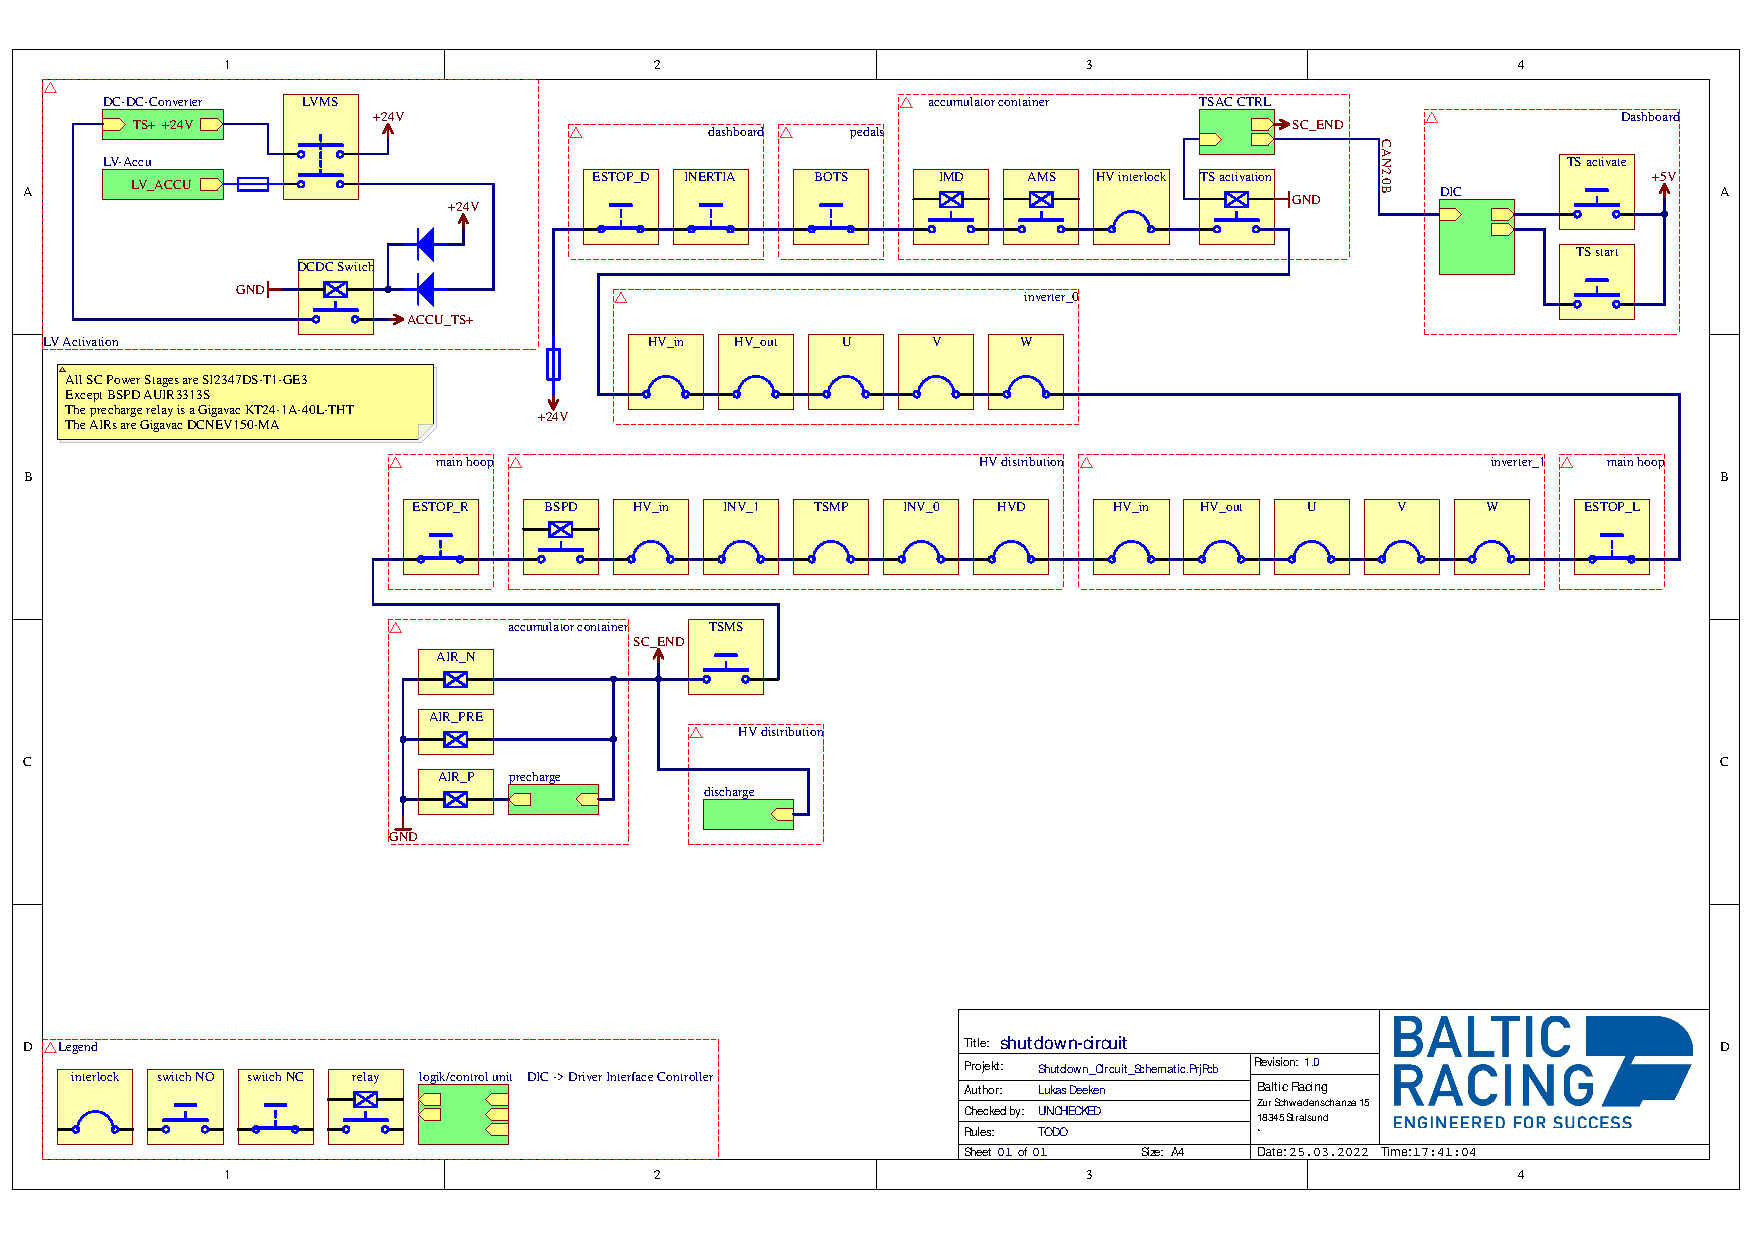
\includegraphics[width=1\linewidth]{bilder/Shutdowncircuit}
	\caption[Shutdown Circuit Schematic]{}
	\label{fig:shutdowncircuit}
\end{figure}

In der obenstehenden Graphic ist der sogenannte shutdown circuit abgebildet. Oben Links befindet sich die Versorgung bzw. der Anfangt des SDC bestehend aus dem Kickstarter für den HVDCDC und der hauptschaltung für das LVMS. Oben rechts befindet sich die TS activation Logik. Im Dashboard des fahrzeuges befinbden sich 2 knopfe, einer um das TS einzuschalten und einer um die Motoren freizuschalten und damit das Losfahren zu ermöglichen. Die kommunikation erfolgt hier über den CAN bus direkt zum AMS Master Auf dem rest des blattes ist von oben nach unten der gesamte shutdowncircuit mit all seinen elementen abgebildet. Am ende des Shutdown circuit befinden sich die AIR welche direkt vom SDC betrieben werden müssen. Weiterhin wird dort das SDCEND Signal abgezweigt welches den ausgangsstatus des SDC abzweigt und z.b dem Discharge bereitstellt.\\
\\
Wichtig beim Shutdowncircuit zu beachten ist das an möglichst vielen stellen stichleitungen eingebracht werden um den SDC an möglichst vielen stellen überwachen zu können. Dies hilft enorm bei der Fehlereingrenzung. Weiter sollter der Querschnitt der Kabel nicht zu dünne gewählt sein. Der Strom im Shutdown Circuit liegt bei ca. 0.24A Da hierrüber ja die AIRs direkt mgeschaltet werden müssen und der SDC hat am ende eine beträchtliche länge im Fahrzeug. 

\subsection{Kabeldimensionierung}
Bei Der Kabeldimensionierung wurden 2 unterschiedliche Ansätze angewandt. Einmal die dimensionierung nach DIN VDE 0298-4 und einmal anhand einer generischen Tabelle. Zweiteres empfiehlt sich eigentlich standardmäßig für so gut wie alle Anwendungen. Ersterer ist hierbei idr nur für soetwas wie die Stromführenden HV Leiter sinnvoll anzuwenden. Die Querschnitberechnung ließe sich mit einem physikalischen Modell noch weiter treiben auf dies wurde jedoch aufgrund des zeitmangels verzichtet.
Folgend ist einmal die bisher verwendete tabelle aufgeführt. Die Quelle der Tabelle war http://www.learn-about-electronics.com/ allerdings ist dies mittlerweile nicht mehr aufzufinden
Bei der Tabelle ist zu beachten das die Ströme für Chassis Wiring verwendet werden. Unter Power Transmission versteht man hier leiter die Mit geringen verlusten z.b in einer industriellen umgebung ströme über lange wege z.b. von Haus zu Haus leiten sollen.
\begin{figure}[h]
	\centering
	\includegraphics[width=0.7\linewidth]{"bilder/Wire thickness"}
	\caption{Leiterquerschnitttabelle}
	\label{fig:wire-thickness}
\end{figure}

Nun soll im Anschluss einmal die Berechnugn der Querschnitte nach DIN VDE 0298-4 (Anhang) dargestellt werden.

Nach 9.4 können wir für ungleichmäßige Ströme den Quadratisdchen Mittelwert zur Leiterquerschnittsbestimmung anstezen. Den Quadratiscvhen mittelwertes des Stromes der Elektromotoren erhalten wir indem wir das mittlere Drehmoment am elektromotor bestimmen, hierfür müssen wir auf die Daten aus der Rundenzeitsimulation zurückgreife, in zukunft empfiehlt es sich die einmal mit den Daten aus dem tatsächlichen fahrzyklus nachzurechnen. Das Drehmoment was wir hier erhalten liegt bei 68,2Nm pro Motor. Im Handbuch des Emrax 208 (Anhang) befindet sich ein Parameter der uns den RMS Strom in A pro NM Drehmoment an der ausgangswelle angiebt. dieser liegt bei 0,8 Nm/A\textsubscript{RMS}. \\
Damit lässt sich ermitteln das der Quadratisdchen Mittelwert des Stromes bei ca. 85,3 A liegt
Nun lässt sich mit hilfe von Tabelle 9.2 der Strom für den Verlegungstyp E (Verlegung wie Motorleiter) für verschiedene Kabelquerschnitte ermitteln Wir ermittlen für 16mm\^2 einen Strom von 80A für 3 belastete Leiter und für 25mm\^2 respektive einen Strom von 101A. Zur sicherheit wurde hier an der stelle auf 25mm\^2 zurückgegriffen, allerdings sollten zukunft durchaus mal versuche mit 16mm\^2 für die Motorleiter unternommen werden da dies zu einer durchaus signifikanten gewichstersparnis führen kann.\\
\\
Für den DC Bus wurde das gleiche vorgehen angewandt. Hier bekommen wir den Strom direkt aus der Rundenzeitsimulation mit 53A. Das ergibt nach Typ E mit 2 belasteten Leitern 10mm\^2 Querschnitt. Jedoch konnten wir keine Steckverbinder finden welcher 10mm\^2 Kabel akzeptiert und ein entsprechendes Rating hat weshalb wir hier auf 16mm\^2 und damit einen max. Strom von 80A gegangen sind. Auch hier gilt wieder das noch Möglichkeiten der Gewichtsersparnis bestehen.\\
\\
\subsection{Hochvolt Kabelbaum}

\begin{figure}[h]
	\center
	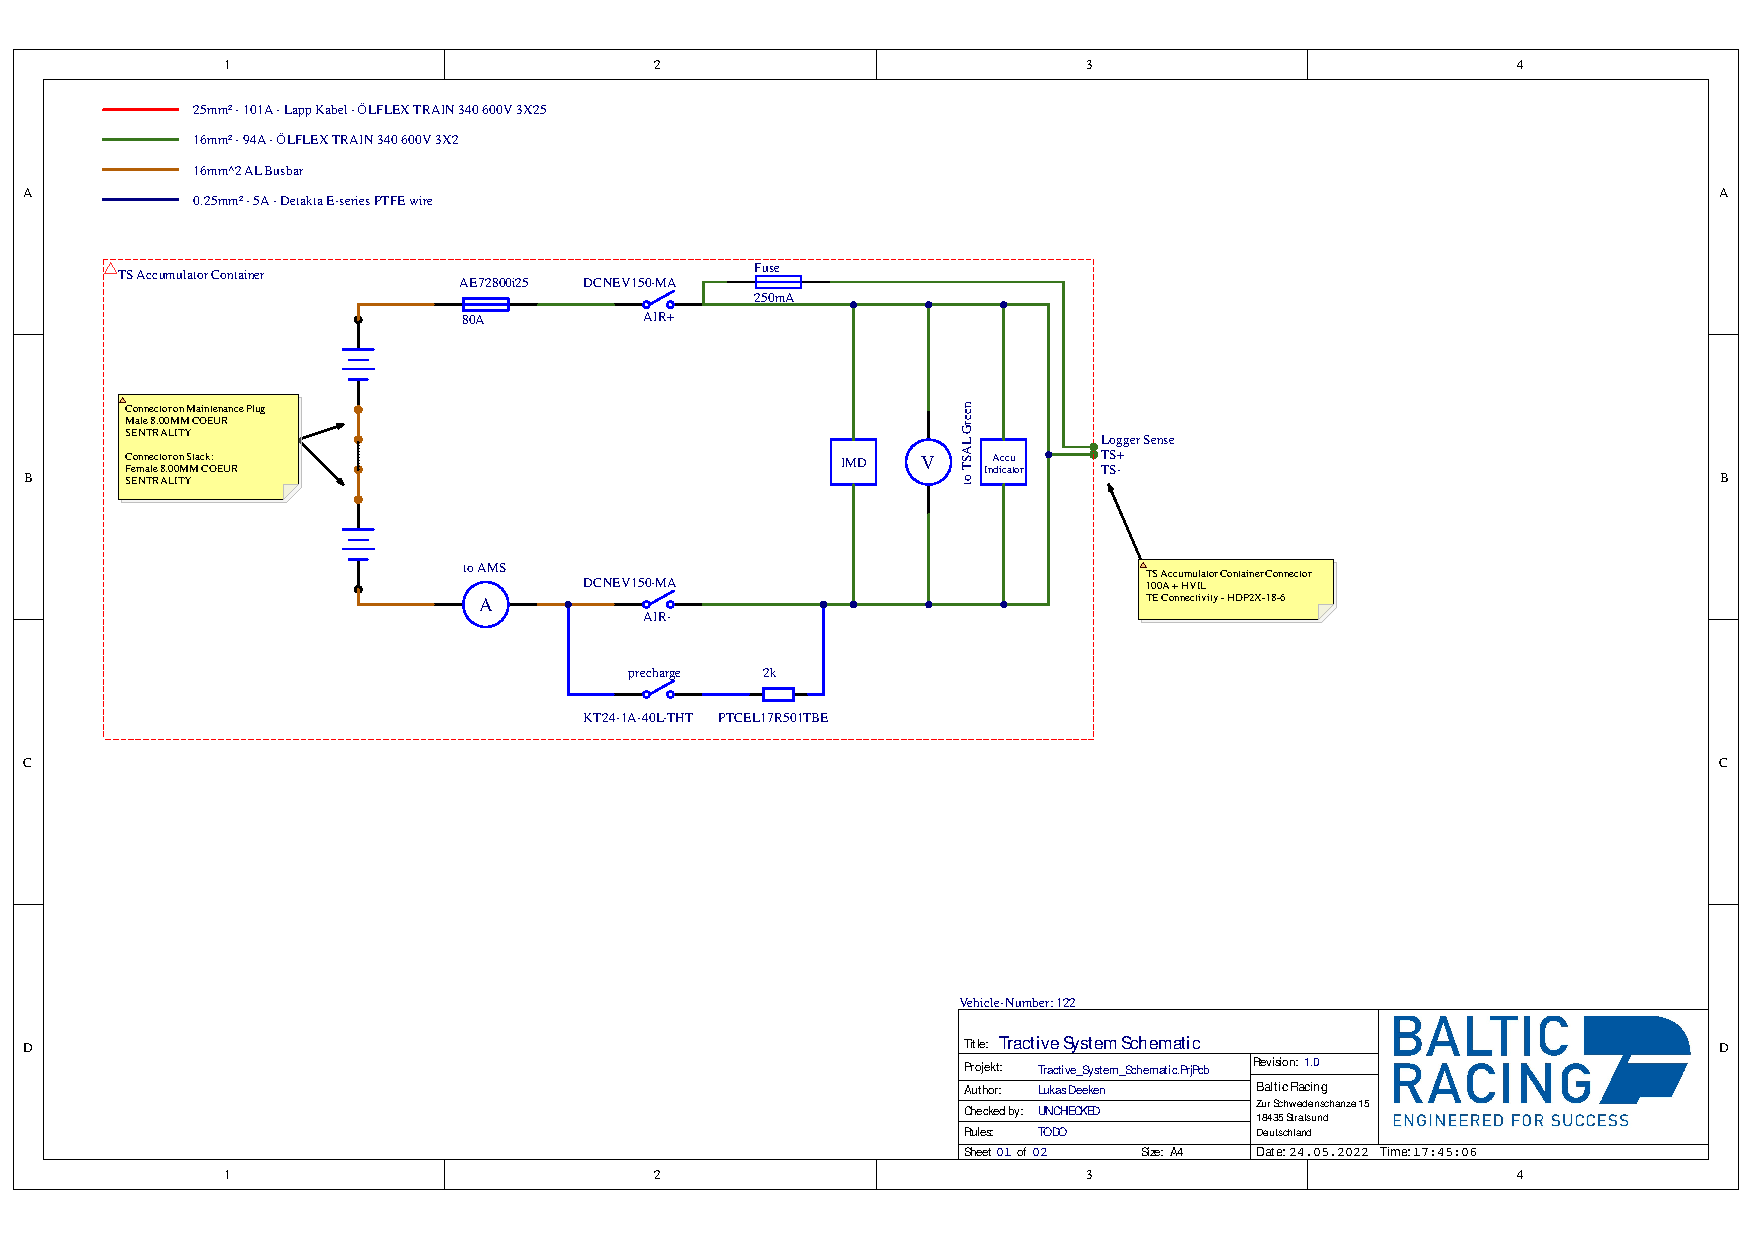
\includegraphics[page=1,width=1\linewidth]{bilder/Tractive_System_Schematic_V4.pdf}
	\caption[Tractive System Schematic]{}
	\label{fig:tractivesystemschematic1}
	
	\center
	\includegraphics[page=2,width=1\linewidth,]{bilder/Tractive_System_Schematic_V4.pdf}
	\caption[Tractive System Schematic]{}
	\label{fig:tractivesystemschematic2}
	\end{figure}

Der HV Kabelbaum besteht aus 3 Kabelsträngen, einer befindet sich innerhalb des Akkus, einer innerhalb der HV Distribution und einer verbindet diese beiden Geräte sowie die Motoren und die Inverter miteinander.\\
\\
Wichtig zu beachten ist das alle HV Kabel Orange und entsprechend isoliert sein müssen. Außerdem dürfen HV und LV Kabel nicht zusammen verlegt werden bzw. sollte es der Fall sein müssen die LV Kabel auch nach HV Spezifikation isoliert sein.
Es gilt besondere Achtsamkeit bei den Leiterquerschnitten sowie den Mindestbiegeradien an den Tag zu legen. Bei den Steckern ist besonders das Voltage Rating Problematisch da hier gerne nur das AC oder DC Rating gegeben wird und hier dann entsprechend umzurechnen ist oder wird. Hierbei wird das AC Rating mal 1.41 gerechnet um das korrespondierende DC Rating zu erhalten. \\
\\
Bei den HV Leitern ist die Möglichkeit von Aluminium Leitern interessant. Hier wurde damals von der Firma Coroflex die zusage gemacht das sollte ein Auftrag für ein derartiges kabel reinkommen würde man für das team eine entsprechende menge kostenlos mit fertigen. Evtl. ließe sich hier in zusammenarbeit mit anderen teams eine nennenswerte menge abnehmen so das sich dir produktion für ein unternhemen lohnt.Hierbei allerdings beachten das die bisherige dimensionierung nur für CU kabel gilt und dementsprechend im besten fall nocheinmal mit dem Unternehmen zusammen durchgeführt werden sollte.\\
\\
Ansonsten gilt zu beachten das man gerade diese Mehradrigen Kabel, sprich kabel mit 3 malö 25mm\^2, wie sie dieses Jahr verwendet werden nicht serienmäßig in orangener Ausführung bekommt was bedeutet das man das Kabel auf jeden Fall einmal in orangenen Schrumpfschlauch einschrumpfen muss. In diesem Zuge wurde bei diesem fahrzeug auch die Schirmung um die kabel selbst eingebracht da dies im gegensatz zur kommerziellen lösung eine gewichtsersparnis von ca. 1kg brachte. Außerdem sollten jegliche stellen wo die isolierung der HV kabel verletz wird z.b an kabelschuhe etc. immer ein Schraumpfschlauch mit innenkleber angebracht werden. es empfehlen sich besonders schläuche mit einem Schrumpfungsverhältnis 3:1. Hierbei gilt zu beachten das es diese schläuche idr. auch nicht in Orange gibt weshalb in dem fall immer ein klebeschrumpfschlauch als auch ein orangener angebracht werden sollte. Für die mehradrigen kabel wurde sich entschieden das diese insgesamt eine gewichtsersparnis bringen und am ende für ein deutlich saubereres und ordentlicheres Gesamtbild sorgen. Bei der Monatge der HV Leiter ist zu beachten das alle verbindungen bei der montage wie z.b. die verschraubung der kabelschuhe an die TSMP fotografiert werden bevor sie in schraumpfschlauch etc. eingepackt werden. Dies ist für die technische abnahme notwendig damit der Prüfer die saubere montage der verbidnung überprüfen kann ohne das etwaiger schrumpfschlauch weider entfernt werden muss. Weiterhin hat isoband im bereicht HV absolut keine sichere Wirkung und wird auch von der FSG nicht als adequater isolator angesehen. Für alle verbindungen etc. gilt stets diese nach datenblatt zu machen. Heißt wenn beim TSMP steckverbinder eine schraube und eine Mutter dabei sind dann werden diese verwendet und nicht irgendwelche Mechanismen zur Schraubensicherung erdacht. Weiterhin gilt zu beachten das jeder einzelne stromführende leiter einzeln abgesichert sein muss, dies erschwert z.b das parallelschalten von mehrern Pins in einem Steckverbinder zum leiten des Stromes da dann am Steckverbinder für jeden parallelen kontakt entsprechende sicherungen vorgesehen sein müssen. Dem aufmewrksamen leser fällt an dieser stelle auf das bei dem Elektromotor in alle drei leitern keine separaten sicherungen vorgesehen sind. Dies lässtr sich darauf zurückführen das der Inverter zugekauft ist und laut datenblatt über einen entsprechendne überstromschutz verfügt. Im Selbstbau Fall müssten hier 3 Sicherungen wie aus dem akku bekannt verbaut werden. 
 
\subsection{Sicherungsauslegung}
Die Sicherung muss stets der schwächste Teil eines Stromkreises sein. In diesem Sinne muss also bei der Auslegung der Stecker darauf geachtet werden das deren Rating höher ist als das der Sicherung oder wir müssen im Unkehrschluss schauen das das rating der sicherung niedriger ist als das der anderen Komponenten. Für DC sicherungen mit einer derart hohen betriebsspannung und einem derart hohen kurzschluisstrom reichen die klassischen flachstecjsicherung wei sie im LV bereich zu finden sind nicht mehr aus. Hier müssen z.b sandgefüllte sicherungen verwendet werden. DIe krux dabei ist es den Lichtbogen der sich beim durchbrennen der sicherung bildet zu löschen. Dies ist bei einer typsichen kfz sicherung nicht gegeben. Zum thema Kurschlusstrom, dieser errechnet sich aus dem innenwiederstand des gesamten akkus und der anliegenden spannung. wir rechnen hier immer im schlimmsten fall sprich alle zellen sind was den innenwiederstand angeht eher im niedrigeren bereich und der akku ist voll geladen. Dabei reden weir von 556,75 V Spannung und 0,528 Ohm Innenwiederstand (berechnung des innenwiederstands einfügen 132S 5P 0,02Ohm pro zelle) Daraus ergibt sich ein Kurzschlusstrom von 1054 A. Der Kurzuschlusstrom sollte mit dem rated breaking current vergliechen werden. ist der Kurzschlusstrom niedriger ist die Sicherung geeignet. Dann haben wir bei der Sicherung natürlich das spannungsratimng welches eingehalten werden muss. Auf basis dieser Dtaen kann eine Sicherung bzw. eine Baureihe heruasgesucht werden, in unserem Fall ergaben die recherchen die AE7 EV Fuse von Adler Elektrik. Die Querschnittsberechnung hat ein Kabel von 16mm\^2 und daher 80A ergeben. Diese 80A legen wir auch bei der Sicherung zu grunde. Dies ergibt die AE72800i25. Daraufhin lässt sich im Datenblatt am Zeit-Strom Schaubild ablesen wie Lange die Sicherung bei Unterschieldichen Strömen braucht um auszulösen. Es ergibt sich eine zeit von ca. 400 s bei einem Strom von 150A und eine Zeit von ca. 0,5ms bei Kurzschlussstrom.

\begin{figure}[h]
	\centering
	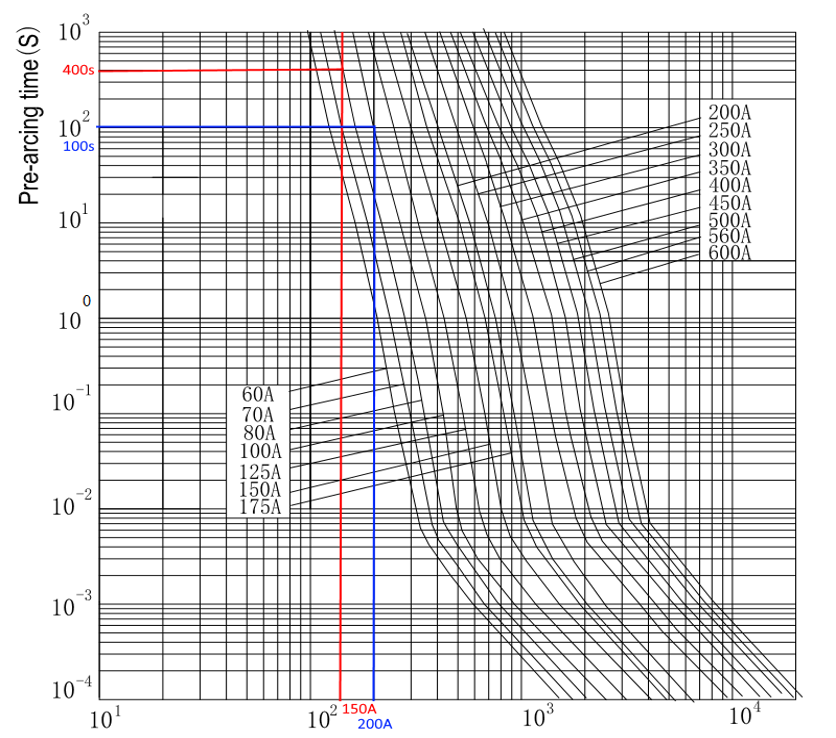
\includegraphics[width=0.7\linewidth]{bilder/Zeit_Strom_TSFUSE}
	\caption{}
	\label{fig:zeitstromtsfuse}
\end{figure}

\subsection{Steckverbinder Auswahl}
Paramter für die Steckverbinder auswahl sind analog zur Kabelauswahl, die betriebsspannung als auch der betriebsstrom. Für informationen hierzu bitte Kapitel xxx refernzieren. Die auswahl der Steckverbinder erfolgt im zuge des Systemdesigns wo die schnittstellen und die anforderungen an diese festgelegt wurden. Der gewählte steckverbdindcxer sollte über ausreichend plätze in der richtigen stärke verfügen um den anforderungen gerecht zu werden. Hierbei ist interessant welche pins man für die steckplätze bekommen kann. oft ist es so möglich so durch unterschieldich große steeckplätze die gleichen kabelquerschnitte zu bekommen. Da es selten steckverbinder gibt die genau zu dem vorliegenden system passen kann dies sehr nützlich sein um das einsetzten eines deutlich größeren und damit schwereren als auch teueren steckverbinder zu verhindern. Auch bei den pins gilt es stets die Stromratings zu beachten. Bei gerade solchen Kabel zu Kabel Verbindern die dazu dienen Kabel in ein Gehäuse zu führen ist es sinnvoll ein paar steckplätze im design frei zu lassen um es zu ermöglichen im nachinein einfach weitere kabel hinzuzufügen sollte dies später einmal notwendig werden. Auch führt das dazu das bei änderung am systemdesign die iunterfaces der Geräte potentiell gleich bleiben können was den test und aufbauprozess des fahrzeuges vereinfacht. 
Bei der Auswahl der steckverbinder ist immer drauf zu achten das entsprechnedes Crimp als auch auspinn bzw. einpinnwerkzeug mit beschafft wird damit die Montage der Verbinder anschließend auch reibungsfrei klappt. Weiter ist auf zusätzliches kabelzubehör wie endkappen blindstecker staubschuzkappen usw. zu achten und mitzubeschaffen. Außerdem ist es üblich die gehäuse der steckverbinder und die Pins separat zu bestellen sodass auch hierdrauf geachtet werden muss. Gerade bei der beschaffung der Pins empfiehlt es sich mindestens um den faktor 1,5 mehr zu bestellen als benötigt da hier öfter ausschuss produziert wird. Auch die steckverbinder können beim Ein bzw. auspinnen kaputt gehen so das man hiervon ersatz vorhalten sollte. 
Eine Besonderheit bei den HV steckern stellt die Interlockleitung dar. Ziel dieser Leitung ist es das HV system abzuschalten sobald ein steckverinder gezogen wird um eoinen elektrischen schlag durch berührenm der kontaklte im steckverinbder zu verhidnern. Hierbei handelt es sich meißt um ein oder zwei weitere Steckkontakte im HV Leiter wo Kabel mit deutlich geringerem Querschnitt angeschlossen werden können. Wichtig hierbei ist das diese interlock leitung aufgehen muiss bevor eine vollständige trennung des steckverbinder (HV Kontakte) erfolgt. 

\subsection{HVD}
Der HVD befindet sich mittig am Heck des Fahrzeuges. Sinn dieses Steckverbinders ist es eine mechanische und damit elektrische Öffnung des HV Systems zwischen Akku und Inverter zu ermöglichen. Dies kann notwendig werden wenn z.b. die Relais im Akku den Dienst verweigern und damit eine Möglichkeit der Trennung der Motoren vom Betriebsstrom anderweitig nicht mehr möglich machen. Bei diesem Steckverbinder kann es sich entweder um dafür vorgesehene Service Trennschalter aus einem regulären Elektrofahrzeug handeln oder um modifizierte Steckverbinder welche auch für den Akku verwendet werden. Die modifizierten sind dabei in der regel kleiner leichter und günstiger.

Bild. verschaltung im auto

\subsection{AIR}
Datenblatt werte, worauf muss ich achten
Break Open Current

Zeichnung zu diesem relai typ

Die AIR`s haben es zum ziel das HV netz des akkus galvanisch vom restlichen fahrzeug zu trennen indem mit einem Relais HV+ und mit dem anderen Relais HV- geöffnet wird. Bei diesen Relais handelt es sich in der regel um, Single Pole Single Throw Normally Open Relais with Auxillary Contacts (SPST NO w AUX). Das heißt wir haben einen Steuerkreis und einen Lastkreis, im stromlosen zusatend ist der lastkreis geöffnet und wir haben einen vom Lastkreis getrennten Kreis welcher synchron zum lastkreis geschaltet wird und somit eine Überwachung des Schaltzustandes des Lastkreises ermöglicht. 
Bei der Auswahl des Relais ist auf das spannungsrating als auch das Stromrating zu achten, aber auch auf die Schaltspannung sprich die spannung des steuerkreises. Weiter ist der schaltsrom ein interessantes kriterium, da es sich bei solch einer Relais spule um eine Induktive last handelt liegt ein recht hoher einschaltstrom vor welcher vom speisenden netzt getragen werden können muss, in unserem vom SDC. Für den TY22 wurde das DCNEV150-M von Littlefuse gewählt.

\section{Ladesystem / Handcart} (zusammen mit Flo Irle)
Charger Schematic erklären
ladegerätauswahl (Ladeleistung)

Das Handcart dient einerseits zum transport des akkus außerhalb des fahrzeuges als auch zum laden des Akkus. Die auswahl des ladegerätes beschränkte sich an der stelle auf ein gerät welches wir von der Firma Schulz elektronik kostenlos bekommen konnten. Hierbei ist dennoch zu beachten das dieses gerät die ladeschlussspannung erreichen kann sprich 600+ Volt abbilden können sollte, als auch über ein programmierbares steuerinterface verfügen sollte, so das eine automatisierte laderegelung ermöglicht wird. Weiter ist die leistung des gerätes interressant, mehr ist hierbei erstmal besser wobei 15Kw mehr als ausreichen sollten da hiermit ein 7,5KWh AKku in 30min geladen werden können sollte. mehr ist an der stelle vom Akku des Rennwagens mit dem aktuellen stand der Technik kaum zu erwarten. 
Beim dem Design des handcartes ist sowohl in elektrischer als auch mechanischer hinsicht auf regelkonformität zu achetn. EInerseits gibt es reglementierung für die maximalen mechanischen abmaße als auch der einsatz einer totmannbremse. andererseits muss das handcart wie das fahrzeug über TSMP, IMD Licht uvm. verfügen. Besondere anforderung ist hierbei das beim laden der satus des akkus ausgegeben werden können muss. Heißt die Spannung als auch die temperatur der zellen muss anzeigbar sein. Dies ist beim TY22 über eine USB verbindung von einem Raspberry Pi zum AMS geplant. Der raspi ist dabei mit einem Touchdisplay ausgesattet und ermöglich so ausgabe der AMS daten als auch steuerung des ladevorganges. Zu guter letzt ist zu beachten das das ladegerät mit in den SDC eingebunden werden muss. Dies erfolgt beim Handcyrt für den TY22 über einen abgrif des SDC end dignales und eine hierüber erfolgende ansteuerung eines relais welche die interlock leitung des ladegerätes öffnet oder trennt. Ein trennen dieser leitung führt laut dastenbaltt zu einem unmittelbaren herunterfahren des ladegerätes.

\begin{figure}
	\centering
	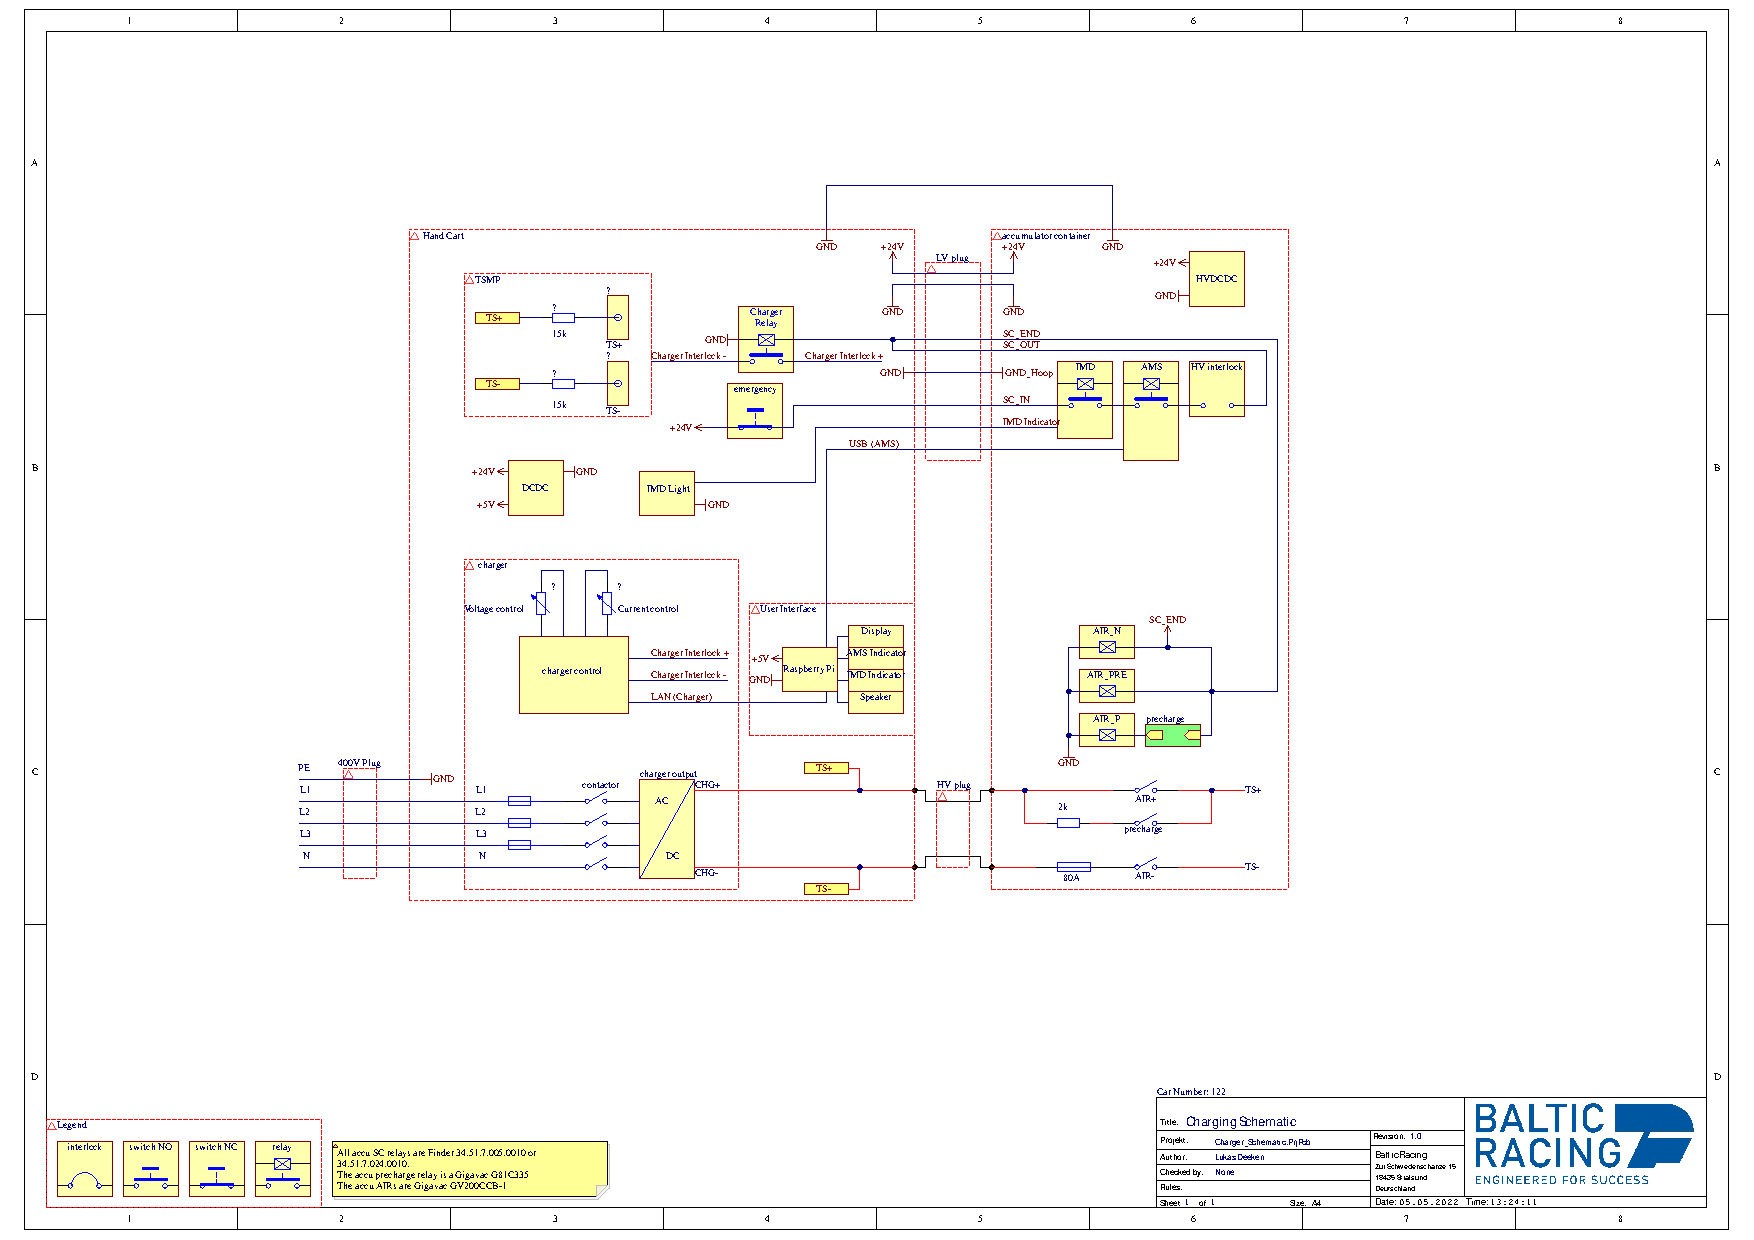
\includegraphics[width=1\linewidth]{C:/Users/lukas/Desktop/Charger_Schematic_V3}
	\caption{}
	\label{fig:chargerschematicv3}
\end{figure}


